% This file should be replaced with your file with thesis content.
%=========================================================================
% Authors: Michal Bidlo, Bohuslav Křena, Jaroslav Dytrych, Petr Veigend and Adam Herout 2019

% For compilation piecewise (see projekt.tex), it is necessary to uncomment it and change
% \documentclass[../projekt.tex]{subfiles}
% \begin{document}

\chapter{Introduction}\label{Introduction}


    Air traffic control (ATC) is an important service provided by control towers which direct aircraft traffic. The proper directions are needed in order to evade collisions, organize the traffic flow and provide useful information for pilots. To ensure that voice communication is clear and quick, a~reliable method needs to be applied. This process can be quite challenging due to an inevitable noisy environment on the pilot side. 

    Some of the most used systems in ATC are very high-frequency radio systems. These systems allow pilots and control towers to communicate in a~certain frequency range. When a~participant in the communication wants to communicate, a~simple press of a~push-to-talk button sets the radio system to transmission mode. By default, the radio system is in receiving mode. Various reliable methods are used for voice activity detection, and many other new approaches can outshine them. 

    The main motivation for this thesis sources from the ATCO2 project, which aims at developing a~platform where air-traffic control data are collected, organized and pre-processed. The main goal of this thesis is to improve the automatic detection of push-to-talk in order to enhance the process of generating segments from captured communication. This could provide an advantage for machines to be able more quickly and accurately process the data. 

    This work will implement automatic detection of voice activity and push-to-talk with the usage of machine learning. In the process of creating a~tool which could correctly detect the speech segments and push-to-talk events, two architectures are proposed and experimented with. The first proposed architecture is a~simple feed-forward neural network whose main purpose was to get acquainted with machine learning. The second proposed architecture is a~two-dimensional convolutional neural network, which provides an upgrade from the first architecture by using convolutional filters which are more suitable for voice activity detection and feature detection overall.

    These models will be trained to detect speech segments and push-to-talk events on the audio recordings provided by the ATCO2 project. The dataset contains files with labels for speech and non-speech segments, which are used to provide supervision during the training of neural networks. 

    The labels for push-to-talk were not provided in the dataset and there are no public implementations for push-to-talk detection, so an algorithm was proposed. This algorithm called \textit{Push-to-talk Event Extraction and Keying} (PEEK) can correctly detect push-to-talk events and has very high accuracy. 
    
    After training and evaluation of the proposed neural networks, the GPVAD implementation was adapted to be fine-tuned on the push-to-talk signals dataset. The GPVAD neural network can with high accuracy detect speech and non-speech segments, and knowledge of this model will be utilised. The GPVAD architecture is trained to detect the push-to-talk by training the whole model and provides very accurate results. 

    The proposed models perform well on the ATCO2 dataset, as they are capable of detecting speech segments and push-to-talk events with high accuracy. 

    In the first chapter, it will be explained what neural networks are and how are they trained. The various architectures are described and discussed. The second chapter provides an overview of the main terms used in this thesis, such as voice activity detection and push-to-talk. Later, the data augmentation techniques and creation of the dataset will be discussed. Finally, the two remaining chapters will explain the process of training the neural networks. The models will be evaluated and compared. 
    
%=========================================================================

\chapter{Neural Networks}\label{ANN}

Just as the human brain processes information and learns from experience, \textit{Artificial Neural Networks} (ANNs) can be thought of as a~digital brain that emulates this process to recognize patterns and make predictions, making them a~powerful tool for solving complex problems. In this chapter, ANNs and their role in machine learning will be examined. The process of designing and training ANNs will be discussed, as well as the various types and architectures explored. The focus of this chapter will be on the practical applications of ANNs, with a~particular emphasis on their use in feed-forward neural networks, convolutional neural networks, and convolutional recurrent neural networks, as they are the core network types used in this work.

\section{Feed-Forward Neural Networks}

\textit{Feed-forward neural networks} (FNNs) \cite{Goodfellow-et-al-2016, aggarwal2018neural, Haykin2004}, also \textit{called multi-layer perceptrons} (MLPs), are a~type of artificial neural network in which nodes do not form loops. The nodes receive data through input nodes, which flow through \textit{hidden layers} and exit through output nodes. The information in the network is only passed forward, and no links exist that allow information to flow back from the output node. 

The FNN approximates functions by calculating classifiers using the formula $y = f^*(x)$, where the input $x$ is assigned to its corresponding output $y$. For instance, in a~classification problem, $f$ could be defined as assigning a~category label to the input being classified. The network establishes a~mapping function:

\begin{equation}\label{mapping}
y = f(x; \theta)
\end{equation}

\begin{itemize}
    \item $\mathbf{x}$ is the input feature vector,
    \item $\mathbf{y}$ is the network's output vector,
    \item $\mathbf{\theta}$ represents the network's learned parameters.
\end{itemize}

The network's goal is to learn the optimal $\theta$ values that result in $f$ approximating the target function $f^*$ as accurately as possible. 

\newpage

In a~simplified form, the feed-forward neural network can be represented as a~\textit{single-layer perceptron} \ref{fig:perceptron}. The single-layer perceptron multiplies input with weights as they enter the layer, and the computed values are summed together. If the sum is above a~certain threshold, typically above zero, the output value is usually converging to one. If the sum falls below the threshold, the output is usually converging to minus one. This behaviour can be found in \textit{Sigmoid} function. This feed-forward architecture is often used for classification, and machine learning algorithms can be integrated into it. 

    \begin{figure}[ht!]
        \centering
        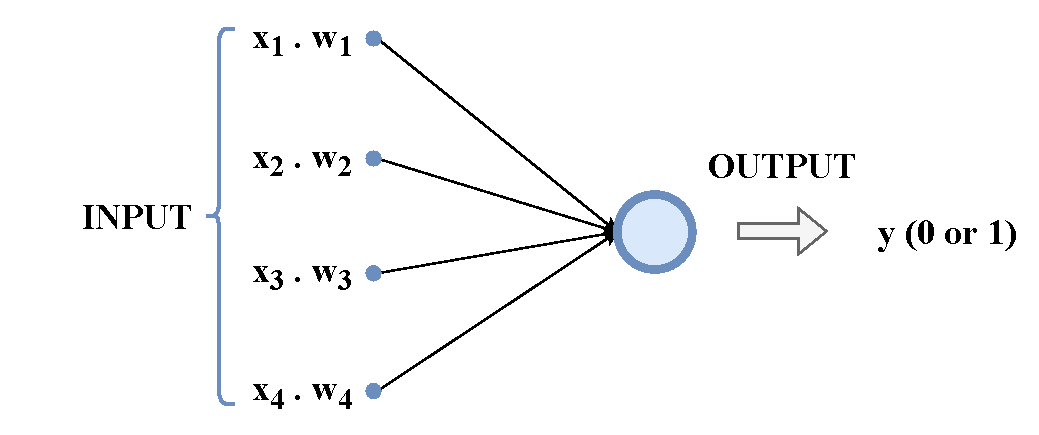
\includegraphics[width = 0.8\textwidth]{obrazky-figures/perceptron.pdf}
        \caption{\textbf{Single-layer perceptron:} computational model that can learn to make decisions based on input data by adjusting weights associated with each input and applying an activation function to produce a~single output.}
        \label{fig:perceptron}
    \end{figure}

\subsection{Layers of FNNs}

Feed-forward neural networks consist of an input layer, one or more hidden layers, and an output layer as shown in figure \ref{fig:layers}. The neurons in the input layer receive input and pass it on to the other layers of the network. The number of neurons in the input layer should match the number of features or attributes in the dataset.

    \begin{figure}[ht!]
        \centering
        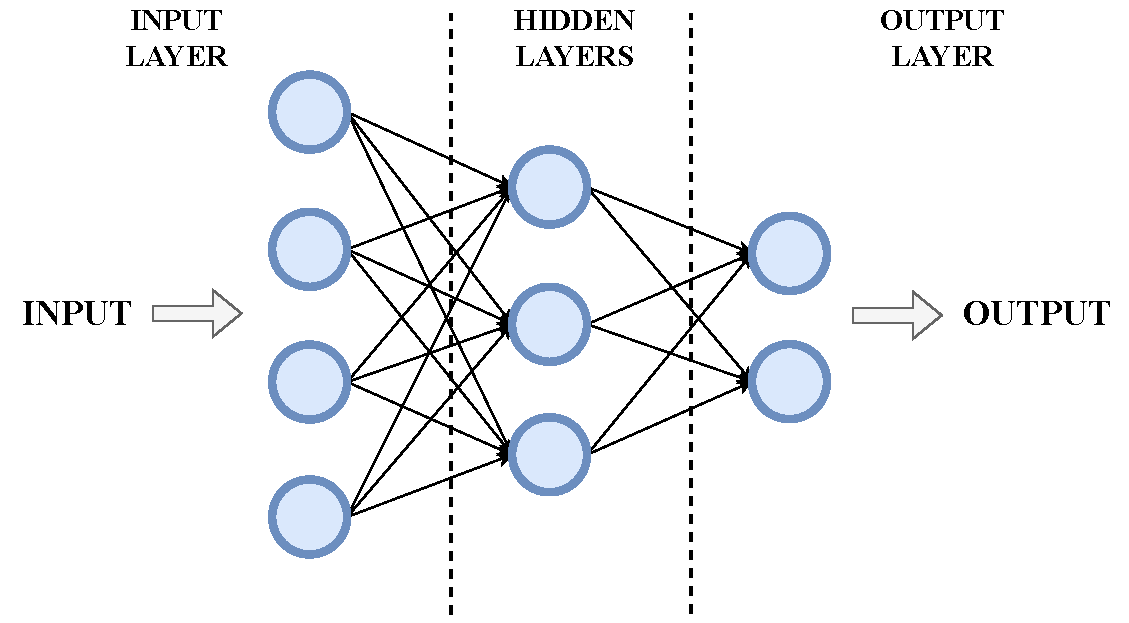
\includegraphics[width = 0.85\textwidth]{obrazky-figures/layers.pdf}
        \caption{Basic FNN structure.}
        \label{fig:layers}
    \end{figure}

\textit{The hidden layers} are placed between the input and output layers and contain several neurons that transform the input before passing it to the next layer. Each neuron in a~layer is connected to the neurons in the previous layer via a~weight, which measures their strength or magnitude. The neuron transforms its input, $x$:

\begin{equation}\label{weights}
f(x; w, b)=w^T \cdot x+b
\end{equation}

\begin{itemize}
    \item $\mathbf{w}$ is a~vector of input weights,
    \item $\mathbf{b}$ is the bias.
\end{itemize}

The weights of the neurons are constantly updated during the learning phase to improve the accuracy of predictions.

\textit{The output layer} represents the forecasted feature, and each neuron in the output layer is connected to the neurons in the last hidden layer. Artificial neurons in feed-forward networks are adapted from biological neurons and function in two ways: creating weighted input sums and activating the sums to make them ``normal''\footnote{After creating the weighted input sums, the neuron applies an activation function to the sum in order to map the output to a~desired range or state. This allows for nonlinear transformations of the input data and enables the network to learn complex patterns and relationships between inputs and outputs.}.

Each \textit{hidden layer} applies an \textit{affine transformation} to its input:

\begin{equation}\label{transformation}
a^n=W^n \cdot z^{n-1}+b^n
\end{equation}

\begin{itemize}
    \item $\mathbf{z}^{n-1}$ is the output vector of the previous hidden layer serving as the input of the current $n$-th layer,
    \item $\mathbf{W}^n$ is a~matrix of weights assigned to the inputs,
    \item $\mathbf{b}^n$ is a~vector of biases assigned to the hidden units,
    \item $\mathbf{a}^n$ is a~vector of output activations.
\end{itemize}

The output of each hidden layer is transformed using a~nonlinear, differentiable \textit{activation function} $h$:

\begin{equation}\label{activation}
z^n=h\left(a^n\right)
\end{equation}

\begin{itemize}
    \item $\mathbf{z}^n$ is the final output of the layer.
\end{itemize}

Neurons in a~neural network make decisions based on the \textit{activation function}, which determines whether a~\textit{linear} or \textit{nonlinear} decision should be made. The activation function also helps to prevent the cascading effect from increasing neuron outputs. This work will specifically use three activation functions (see figure \ref{fig:activ}): Sigmoid, ReLU, and LeakyReLU. These activation functions are used for regression problems.

    \begin{figure}[ht!]
        \centering
        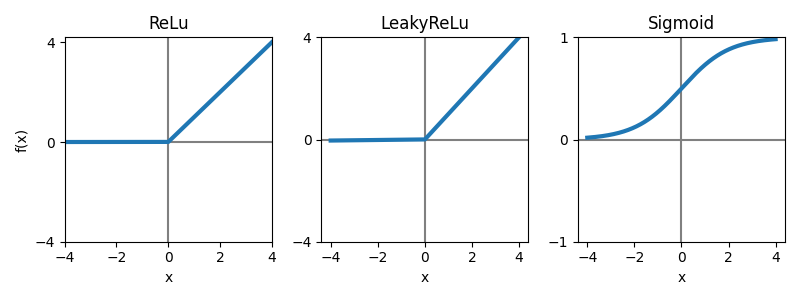
\includegraphics[width = \textwidth]{obrazky-figures/active.png}
        \caption{Graphic representation of activation functions: Rectified Linear Unit (ReLU), LeakyReLU and  Logistic Sigmoid (Sigmoid) activation functions.}
        \label{fig:activ}
    \end{figure}

\newpage

In FNN, the choice of activation function is important and depends on various factors. The activation function used in the output layer (such as logistic \textit{Sigmoid}) is often different from the one used in the hidden layers. The \textit{rectified linear unit} (ReLU) has become a~popular choice for hidden layers, due to its simplicity and effectiveness in preventing the \textit{vanishing gradient problem}\footnote{When the gradients in the early layers of a~deep neural network become very small during backpropagation, leading to poor convergence or no convergence at all. This issue can be mitigated by using activation functions like ReLU or other optimization techniques.}. \textit{ReLU} only allows positive values to flow through, while negative values are mapped to 0. \textit{LeakyReLU} is a~variant of ReLU that addresses the ``dying ReLU'' problem\footnote{It happens when the gradient of the function becomes zero or very close to zero for certain inputs, causing the neuron to ``die'' and no longer contribute to the network's output.} by allowing a~small gradient to flow when the input is negative. \textit{Sigmoid} is another popular activation function that squashes the input into a~range between 0 and 1, making it useful for \textit{binary classification} problems. 

Lastly, in the thesis, another activation function is used for the classification problem. \textit{Softmax} activation function is commonly used on output layers to produce a~probability distribution over K classes. This probability distribution is useful in \textit{multi-class classification} problems. 

It is crucial for the activation function to be nonlinear, allowing the network to perform complex transformations beyond affine transformations. This enables the network to bend and fold the input feature space to model class boundaries in complex classification problems.
\newpage
\subsection{The Process of Training the FNN}

    The training process of the neural network starts with proper data preparation, which will be discussed in chapter \ref{Data}. After preparing data, the training can start \cite{applyingnn}. 

    For simplicity, training methods can be divided into three types \cite{hajaj_ml_intro}: 

    \begin{itemize}
        \item \textbf{Supervised learning} is when the neural network is provided true values which are excepted from the trained model. 
        \item \textbf{Semi-Supervised learning} uses labelled as well as unlabelled data to train the neural network.
        \item \textbf{Unsupervised learning} does not require labels and therefore is not provided with any feedback during training. For unsupervised learning, a~method such as clustering is used. 
    \end{itemize}
    
    In this work, only supervised learning is implemented. Both push-to-talk and voice activity detection is trained with labels. 

    Supervised learning can be further divided into two types:

    \begin{itemize}
        \item \textbf{Classification} is a~process when the neural network provides a~prediction of the class to which the input data should belong.
        \item  \textbf{Regression} models predict the specific value as an output.
    \end{itemize}

    In this thesis, the classification method will be used. 
    
    As it was mentioned earlier, the neural network consists of neurons. When training from scratch, the weights and biases are initialised randomly. During the training process, these values change based on provided parameters. These parameters are called \textit{hyperparameters}. They are the most essential in the training process. The most crucial parameters are \textit{learning rate, loss function} and \textit{optimizer}.

    The difference between the predicted output and true value is computed by the chosen loss function. There are various loss functions used for classification problems, but one of the most common is \textit{CrossEntropy} \ref{crossentropyformula}. Every training process explained in chapter \ref{Experiments} uses this loss function. 

    \begin{equation}\label{crossentropyformula}
        H_p(q)=-\frac{1}{N} \cdot \sum_{i=1}^N y_i \cdot \log \left(p\left(y_i\right)\right)+\left(1-y_i\right) \cdot \log \left(1-p\left(y_i\right)\right)
    \end{equation}

    After computing the difference between ground truth and predicted value, it is necessary to optimize weights to assure that the next prediction is closer to ground truth. The predicted output is computed in the \textit{forward pass} by applying weights and activation functions to the input. 

    The modification of the weights and biases is done by the optimizer call. The optimizer is initialised with a~\textit{learning rate}. The learning rate represents the step size at each iteration. It scales down the computed gradients computed during the \textit{backward pass} call. The backward pass is done by \textit{backpropagation} algorithm. 

    Some of the most common optimizers are \textit{Stochastic Gradient Descent} (SGD)\footnote{see
        \href{pytorch.org/docs/stable/generated/torch.optim.SGD.html}{\texttt{pytorch.org/docs/stable/generated/torch.optim.SGD.html}}} or 
    \textit{Adaptive Moment Estimation} (Adam)\footnote{see \href{https://pytorch.org/docs/stable/generated/torch.optim.Adam.html}{\texttt{pytorch.org/docs/stable/generated/torch.optim.Adam.html}}}, 
    \textit{Adaptive Moment Estimation with weight decay} (AdamW)\footnote{see
    \href{pytorch.org/docs/stable/generated/torch.optim.AdamW.html}{\texttt{pytorch.org/docs/stable/generated/torch.optim.AdamW.html}}}.

    SGD is a~simple optimization algorithm for training neural networks that update weights based on the gradients. Adam and AdamW are extensions of SGD that can adaptively adjust learning rates and introduce weight decay to improve training performance.

    The outcome of the training process depends on other important parameters \cite{aaltonn} such as \textit{Batch size}, and number of \textit{Epochs}. 
    
    \textit{Batch size}, encapsulates input to a~vector of batch size. These chunks can make the model more generalised.

    \textit{Epoch} represents a~single training iteration of all batches in both forward and backward passes. Setting the number of epochs too high could lead to \textit{overfitting}. This would restrain the model from learning how to generalise the data, but rather perfectly fit the training data.

    To prevent overfitting of the model, \textit{Regularisation techniques} are applied. Regularisation techniques such as \textit{dropout} and \textit{batch normalisation} do not only prevent overfitting, but can also improve the accuracy of the model. The dropout method drops a~number of neurons in the hidden layers. Randomly setting to zero some of the neurons forces other neurons to learn to recognise features. The batch normalisation method normalises the input layer to range from zero to one to speed up training.  


\section{Convolutional Neural Networks}

\textit{Convolutional Neural Networks} (CNNs) \cite{Goodfellow-et-al-2016, aggarwal2018neural} are a~type of neural network that is well-suited for processing and analysing data that has a~grid-like structure, such as images, audio, and time-series data. Unlike FNNs, CNNs have connections that are sparse and shared. These connections reduce the number of parameters in the network and make it possible to process large amounts of data more efficiently.

The basic idea behind CNNs is to use a~set of learnable filters, also called kernels or weights, that slide over the input and compute \textit{dot products}\footnote{The mathematical operation that takes two vectors of equal dimensionality and returns a~single scalar value.} between the weights and the local regions of the input. This operation is known as \textit{convolution} and produces a~\textit{feature map} that highlights certain features or patterns in the input. 

\newpage

The convolution operation can be represented as follows:

\begin{equation}\label{convolution}
S(i,j) = (I * K)(i,j) = \sum_m \sum_n I(m,n) \cdot K(i-m,j-n)
\end{equation}

\begin{itemize}
\item $\mathbf{S}$ is the output feature map,
\item $\mathbf{I}$ is the input,
\item $\mathbf{K}$ is the filter or kernel.
\end{itemize}

Each neuron in the feature map is connected to a~small patch of the input and shares the same weights, which are learned during training. This weight sharing reduces the number of parameters in the network and allows CNNs to learn translation-invariant features.

\subsection{Layers of CNNs}

CNNs are composed of multiple layers that are arranged in a~specific order, for example, shown in figure \ref{fig:CNN_layers}.

    \begin{figure}[ht!]
        \centering
        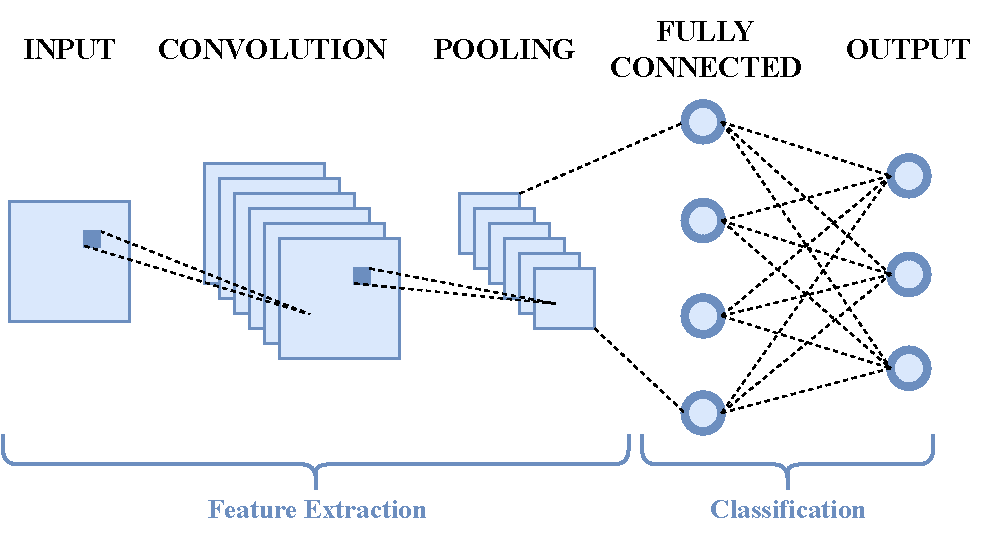
\includegraphics[width = \textwidth]{obrazky-figures/CNN_layers.pdf}
        \caption{An illustration of the regular CNN for signal processing.}
        \label{fig:CNN_layers}
    \end{figure}

\textit{Convolutional layers} are the core building blocks of CNNs. They apply several \textit{filters} or \textit{kernels} that slide over the input and perform a~convolution operation. Each filter produces a~\textit{feature map} or activation map, which represents the presence or absence of specific patterns or features in the input.  The output of a~convolutional layer is fed to a~non-linear activation function (such as ReLU), which introduces non-linearity into the network and enables it to learn more complex patterns. The output is then passed to the next layer, which could be another convolutional layer or a~pooling layer. 


\textit{Pooling layers} are used to reduce the spatial dimension of the \textit{feature maps} produced by the convolutional layers. They do this by \textit{downsampling} the input in a~specific window and returning a~single output value. The most common type of pooling is \textit{max pooling}, where the maximum value in the pooling window is selected as the output (see figure \ref{fig:maxpool}). Max pooling helps to reduce the number of parameters in the network and also makes the network more robust to small translations in the input.

    \begin{figure}[ht!]
        \centering
        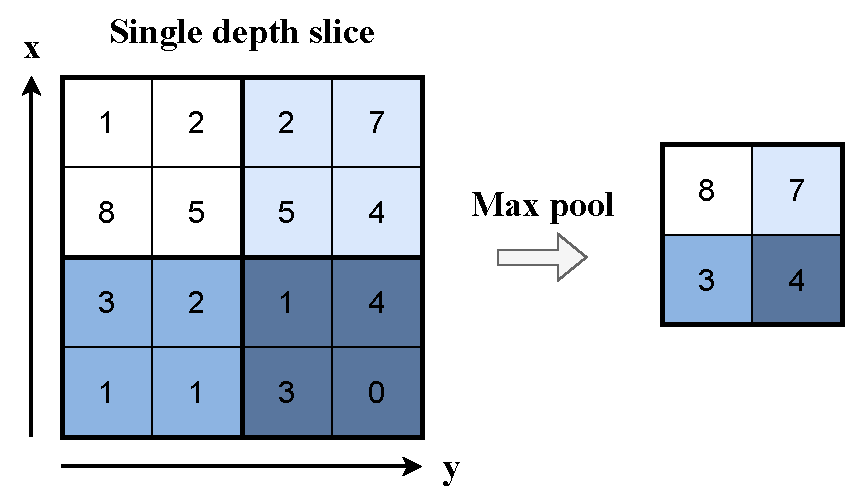
\includegraphics[width = 0.6\textwidth]{obrazky-figures/maxpool.pdf}
        \caption{The process of downsampling an input, using 2×2 filters and moving the filter by a~distance of 2 pixels each time.}
        \label{fig:maxpool}
    \end{figure}

\textit{Fully connected layers} are used to connect all the neurons in one layer to all the neurons in the next layer. They are commonly used as the last layers in CNNs to classify the input into different classes. 


\section{Convolutional Recurrent Neural Networks}

\textit{Convolutional Recurrent Neural Networks} (CRNNs) \cite{shi2015convolutional} combines the power of both convolutional and recurrent layers (see figure \ref{fig:CRNN_layers}). The input is filtered by the convolutional layers, which then create feature maps which bring attention to particular patterns and features. These feature maps are then given to the recurrent layers, which keep a~hidden state that is updated at each time step and so captures the temporal dependencies.

    \begin{figure}[ht!]
        \centering
        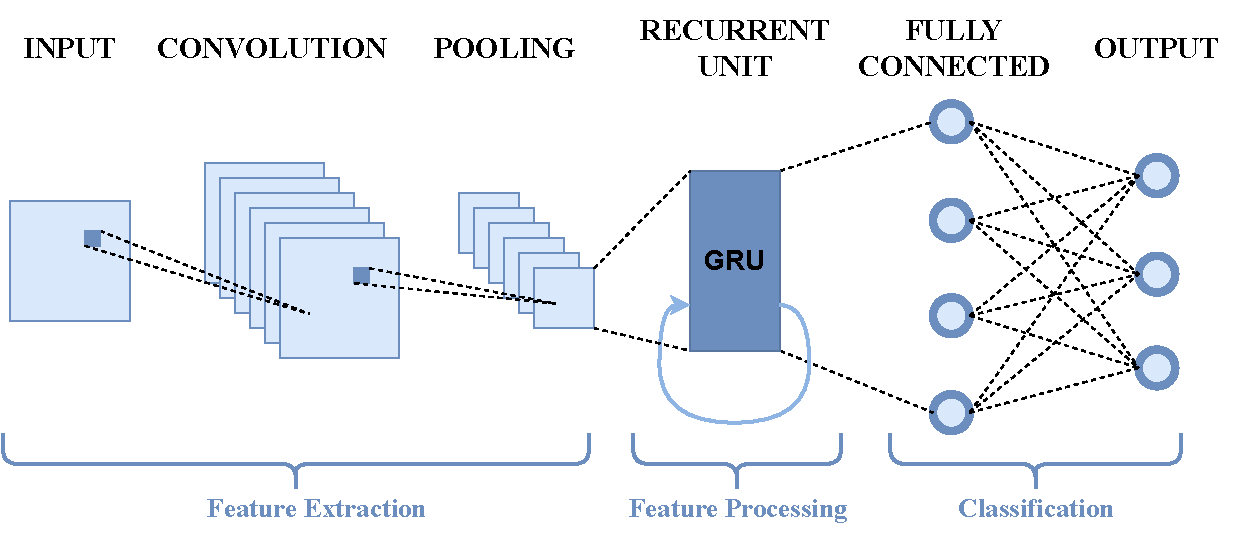
\includegraphics[width = \textwidth]{obrazky-figures/CRNN_layers.pdf}
        \caption{The architecture of simple CRNN.}
        \label{fig:CRNN_layers}
    \end{figure}

\subsection{Layers of CRNNs}

\textit{Convolutional layers} in CRNNs are similar to those in CNNs. They apply filters that slide over the input and produce feature maps. The output of the convolutional layers is fed to the recurrent layers.

\textit{Recurrent layers} model sequential or time-series data, with an emphasis on data order. In contrast to feedforward and convolutional layers, which process each input independently and do not have any memory of previous inputs, recurrent layers maintain a~hidden state that summarizes the previous inputs and influences the processing of the current input.

Utilising a~feedback loop to link the layer's output to its input is the basic concept behind recurrent layers. This feedback loop allows the layer to pass information from one time step to the next and maintain a~memory of the past inputs. In combination with convolutional layers, it allows CRNNs to handle both spatial and temporal information in data such as video or audio.

There are several variants of recurrent layers, including \textit{Long Short-Term Memory} (LSTM) and \textit{Gated Recurrent Unit} (GRU) layers, which use more complex architectures to better handle the flow of information through the network and mitigate the vanishing gradient problem. GRU is part of a~CRNN architecture, that will be discussed in chapter~\ref{Experiments}.

A GRU \cite{DBLP:conf, olah2015understanding} unit typically consists of two gates: a~reset gate and an update gate. The reset gate determines how much of the previous hidden state to forget, while the update gate determines how much of the new information to keep. The output of the GRU unit is a~combination of the previous hidden state and the new candidate state that is computed based on the input and the reset gate.

The mathematical formulation of a~GRU unit can be expressed as follows (see figure~\ref{fig:LSTM3-var-GRU}):
    \begin{figure}[ht!]
        \centering
        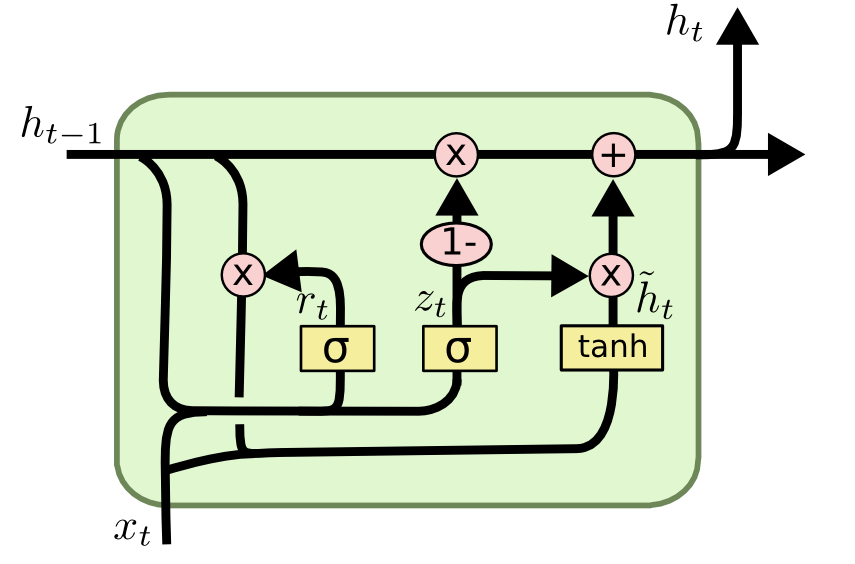
\includegraphics[width = 0.6\textwidth]{obrazky-figures/LSTM3-var-GRU.png}
        \caption{Graphic representation of a~GRU cell. The image was obtained from \cite{olah2015understanding}.}
        \label{fig:LSTM3-var-GRU}
    \end{figure}

\begin{enumerate}
    \item First, we compute the \textit{update gate} \textbf{$z_t$} and the \textit{reset gate} \textbf{$r_t$} using the input \textbf{$x_t$} and the previous hidden state \textbf{$h_{t-1}$},
    
    \begin{equation}
    \begin{aligned}
    & z_t=\sigma\left(W_z \cdot\left[h_{t-1}, x_t\right]\right) \\
    & r_t=\sigma\left(W_r \cdot\left[h_{t-1}, x_t\right]\right)
    \end{aligned}
    \end{equation}

    where \textbf{$\sigma$} is the \textit{sigmoid activation function}, \textbf{$W_z$} and \textbf{$W_r$} are weight matrices.

    \item Next, we compute the \textit{candidate state} \textbf{$\tilde{h_t}$} using the input \textbf{$x_t$} and the \textit{reset gate} \textbf{$r_t$},

    \begin{equation}
    \tilde{h}_t=\tanh \left(W \cdot\left[r_t * h_{t-1}, x_t\right]\right)
    \end{equation}
    
    
    where \textbf{$*$} represents the element-wise multiplication.

    \item Finally, we compute the \textit{new hidden state} \textbf{$h_t$} as a~\textit{linear interpolation} between the \textit{previous hidden state} \textbf{$h_{t-1}$} and the \textit{candidate state} \textbf{$\tilde{h_t}$}, weighted by the update gate \textbf{$z_t$},
    
    \begin{equation}
    h_t=\left(1-z_t\right) * h_{t-1}+z_t * \tilde{h}_t
    \end{equation}

    where \textbf{$*$} again denotes element-wise multiplication.
    
\end{enumerate}
With state-of-the-art performance for many sequential modelling tasks, the GRU is currently one of the most popular and widely used CRNN variations.


\textit{Fully connected layers} in CRNNs are used to connect all the neurons in one layer to all the neurons in the next layer. They are commonly used as the last layers in CRNNs to classify the input into different classes.
 

%=========================================================================

\chapter{Voice Activity Detection and Push-to-talk in Air Traffic Communication}\label{Literature}

Effective communication is crucial for Air Traffic Control operations. To ensure quality and flight safety, advanced signal processing techniques are necessary.
This chapter focuses on two techniques: Voice Activity Detection and Push-to-talk in Air Traffic Communication. Section \ref{ATCon} provides an overview of Air Traffic Control operations and how to execute them safely and timely. 
Section \ref{VAD} discusses the concept of Voice Activity Detection. It explains why this process is necessary and how speech segments are separated from non-speech segments in a~communication channel. 
Finally, section \ref{PTT}, introduces the concept of Push-to-talk, which is used to control speech transmission between two endpoints. 

\section{Air Traffic Control}\label{ATCon}

Air traffic control (ATC) is a~system of technologies and procedures that guide the movement of aircraft in the air and on the ground. ATC is in charge of maintaining aircraft separation, delivering clearances and instructions to pilots, as well as monitoring and directing traffic flow to prevent collisions \cite{CAA}.

The major goal of ATC is to ensure the security of aircraft, passengers, and crew, as well as to avoid collisions with other aircraft and obstructions.
ATC controllers work in control towers or in en-route centres to monitor the movement of aircraft and to communicate with pilots using radar, radio, and computer systems.

\subsection{Air Traffic Communication}\label{ATCom}

Communication between pilots and controllers during different phases of flight is an essential element of air traffic control. This communication follows established protocols and phraseology, including standardized language developed by the International Civil Aviation Organization (ICAO)\footnote{see \href{https://www.icao.int/Pages/default.aspx}{{\fontfamily{cmtt}\selectfont https://www.icao.int/Pages/default.aspx}}}. To guarantee clear communication and reduce misunderstandings and mistakes, pilots and controllers get trained to use standardised phraseology and adhere to established procedures \cite[ch. 1, pp. 18-19]{ATM:2017}.


Standard phraseology is used in different types of communication, including radio communication, which is the primary method of communication between pilots and controllers \cite[ch. 2, pp. 30-31]{ATM:2017}. Radio communication requires the use of specific tools and techniques, such as selecting the right frequency to connect with air traffic control and delivering necessary information in a~simple and straightforward way.


\subsection{Very High-Frequency Channel}\label{VHF}

According to the FAA's ``Air Traffic Control'' guide \cite[p. 573]{faa-atc}, VHF (Very High Frequency) is a~band of radio frequencies between $118.000$ and $136.975$ MHz that is used for short-range communication in air traffic control. VHF is the primary communication method used in ATC and is used for communication between pilots and air traffic controllers on the ground and in the air.

VHF communication is accomplished using a~network of ground-based radio transmitters and receivers that are located at airports and other ATC facilities. Each facility has one or more VHF channels assigned to it for communication with pilots. Pilots tune their VHF radios to the appropriate channel for the facility they are communicating with.

When communicating on a~VHF channel \cite[pp. 53-54]{faa-atc}, pilots and air traffic controllers use standard phraseology to exchange information about the aircraft's position, altitude, heading, and intentions. This information is used by air traffic controllers to safely and efficiently manage air traffic in the vicinity of the airport or in the airspace sector they are responsible for.

VHF is an essential component of air traffic control, providing reliable and efficient communication between pilots and controllers and helping to ensure the safety of the flying public.

\section{Voice Activity Detection}\label{VAD}

% dopisat nieco o VAD v ATC

Voice Activity Detection (VAD) is a~process that's main goal involves identifying speech regions in a~noisy audio signal using a~feature vector $x$ and deciding between two hypotheses~\ref{VADhypotheses} of speech and noise \cite{Ramirez07}. As a~result, each audio frame from the source will be evaluated against:

\begin{equation}\label{VADhypotheses}
    \begin{array}{ll}
    H_0: & x=n, \\
    H_1: & x=n+s
    \end{array}
\end{equation}

\begin{itemize}
    \item $H_0$ hypothesis suggests that the current frame solely contains noise or/and other non-speech signals $n$,
    \item $H_1$ hypothesis indicates that the current frame consists of a~speech signal $s$ and potential background noise signals.
\end{itemize}

Whether a~frame contains speech or noise can be determined by choosing the hypothesis with the highest probability given the current frame's features $x$, using a~method called maximum a~posteriori classification, expressed using Bayes' theorem:

$$
\operatorname{VAD}\left(x\right)= 
    \begin{cases}
        \text { non-speech } & \frac{P\left(x \mid H_0\right) \cdot P(H_0)}{P(x)}>\frac{P\left(x \mid H_1\right) \cdot P(H_1)}{P(x)} \text{,} \\ 
        \text { speech } & \text { else. }
    \end{cases}
$$

When performing voice activity detection, it is common to break down the process into three distinct stages, with each stage playing a~crucial role in determining whether speech is present in an audio signal. These stages typically include:

\begin{enumerate}
    \item \textbf{Feature extraction}, where relevant features are extracted from the audio signal. It is important to take into consideration the approach used for modelling voice activity detection because various methods may require different features;
    \item \textbf{Decision module} where a~decision is made about whether the audio signal contains speech or noise based on the extracted features;
    \item \textbf{Decision smoothing}, to deal with VAD decision errors that may occur due to high levels of background noise. It can help reduce the number of false positive or negative decisions by making the VAD decision less erratic and more dependable.
\end{enumerate}

    \begin{figure}[ht!]
        \centering
        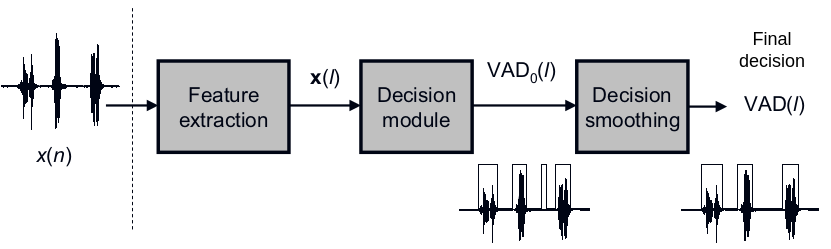
\includegraphics[width = \textwidth]{obrazky-figures/VAD_diagram.png}
        \caption{A graphical representation showing the components and their interconnections of a~VAD system.  The figure was adapted from \cite{Ramirez07}.}
        \label{fig:VAD_diagram}
    \end{figure}
    
VAD is an important preprocessing step in larger speech-processing systems, such as speech recognition, speaker recognition, and speech enhancement. One of the advantages of VAD is that it can reduce the computational cost of speech processing algorithms by removing non-speech segments from the audio signal.

However, VAD can be difficult to implement, especially in loud or acoustically challenging environments in general. Speech and other sounds, such as background noise or music, may be difficult to distinguish, especially when using traditional VAD methods. Machine learning-based approaches may 


\subsection{Traditional Voice Activity Detection Approaches}\label{traditional}

Traditional VAD Approaches date back to the 1970s, and the field has a~long history \cite{Adlin21}. In general, traditional VAD methods involve analysing various characteristics of the input signal and using a~heuristic or specific algorithm to make an accurate decision. These characteristics typically include energy levels, spectral information, zero-crossing rate, and long-term spectral divergence \cite{tanyer2000voice, aaltovad}. The most essential traditional VAD methods include:

\begin{itemize}
    \item \textbf{Energy-Based Method}, which uses the energy level of the speech signal as the primary feature to detect speech activity. The basic idea is that speech signals have a~higher energy level than non-speech signals such as background noise or silence.
    \item \textbf{Zero-Crossing Rate Method's} evaluation is based on the number of times the audio signal crosses the zero-axis in a~given time frame. The concept is that speech signals have a~higher ZCR than non-speech signals, because speech signals contain more rapid changes in amplitude due to the vocal cords vibrating, while non-speech signals, such as background noise or silence, have a~more consistent amplitude.
    \item \textbf{Spectral-Based Method} uses spectral characteristics of speech and non-speech signals to distinguish between them. This method analyses the power spectral density (PSD) of a~signal to extract features that can be used to classify the signal as speech or non-speech.
\end{itemize}

The choice of which VAD method to use may vary depending on the specific context, such as available resources, desired level of accuracy, or system performance requirements.

\subsection{Machine Learning Voice Activity Detection Approaches}\label{modern}
Modern approaches to VAD incorporate machine learning techniques \cite{6857341, aaltonn}, which have become increasingly popular and have begun to replace traditional VAD methods.

Machine learning-based VAD methods involve using statistical and machine learning techniques to learn patterns in audio data that are indicative of speech or non-speech, and then using these patterns to classify new audio samples.

Some common machine learning-based approaches for VAD include:

\begin{itemize}
    \item \textbf{Supervised Learning Methods} for VAD represent training a~machine learning model on labelled data, where the labels denote whether a~given audio segment contains speech or not. The model learns to recognize patterns in the audio that are associated with speech, such as the presence of voiced sounds, energy in a~particular frequency range, or changes in spectral content over time. The model can then be used to classify new, unlabelled audio segments as speech or non-speech.

    \item \textbf{Unsupervised Learning Methods} for VAD involve using clustering techniques to segment the audio into speech and non-speech clusters without relying on labelled data. For example, k-means clustering can be used to group similar segments of audio together based on their spectral properties, or Gaussian mixture models can be used to fit a~mixture of Gaussian distributions to the audio data, with each component corresponding to either speech or non-speech.
\end{itemize}

    \textit{Deep Learning Methods} for VAD involves training deep neural networks (DNNs) on raw audio signals or spectrogram features to perform VAD. Convolutional Neural Networks (CNNs) and Convolutional Recurrent Neural Networks (CRNNs) are commonly used for VAD using deep learning techniques. In a~CNN, filters are applied to small segments of the audio to extract local features, which are then pooled and combined to form higher-level representations. In a~CRNN, the network maintains a~memory of previous time steps and uses this information to make predictions about the current segment of audio.

The exact approach used can depend on factors like the nature of the audio data, the required accuracy and speed of the VAD, and the resources available for model training and deployment.

\subsection{Voice Activity Detection and Air Traffic Control}\label{VADinATC}

Air Traffic Control systems relies heavily on VAD, because it helps to filter out background noise and detect when pilots are speaking. There may be several pilots and air traffic controllers communicating on the same frequency in an ATC environment, which can cause interference and confusion. By identifying speech activity and muting the audio when there is silence, VAD can help reduce these problems.

In emergency situations, it is important for ATC to quickly identify and prioritize communication from pilots. VAD can help to automatically detect when a~pilot is speaking and alert the air traffic controller to the urgency of the situation, enabling them to respond quickly and appropriately.

\section{Push-To-Talk}\label{PTT}

\textit{Two-way radio systems}\footnote{Short-range communication systems that allow multiple parties to communicate using radio waves.} receive and transmit signals through very high-frequency waves~\cite{tallman_ptt_switch_2021}. To transmit audio, a~push-to-talk switch needs to be pressed. By pressing and holding, the communicant can start to speak. Depending on the specific system, this event can produce a~``click'' sound. Without pressing the switch, the communication channel is in receiving mode. 

The start of the push-to-talk event begins with pressing the button. This action sends an electrical signal to the device, which activates the microphone and broadcasts the audio as an analogue signal. The signal can be in the real-time heard by the listener on another headset. The push-to-talk event can be identified as a~sudden change in voltage. Figure \ref{fig:ptt} shows audio with a~noticeable push-to-talk event. The red square represents the duration of this event that was selected for this thesis. The duration of the PTT event is approximately $100$ ms long.

There are little to no public implementations on how to detect push-to-talk events, so comparison with different approaches is not possible. The push-to-talk duration is at least $100 ms$. The position of the peak is usually at the beginning of the frame sequence. 

    \begin{figure}[ht!]
        \centering
        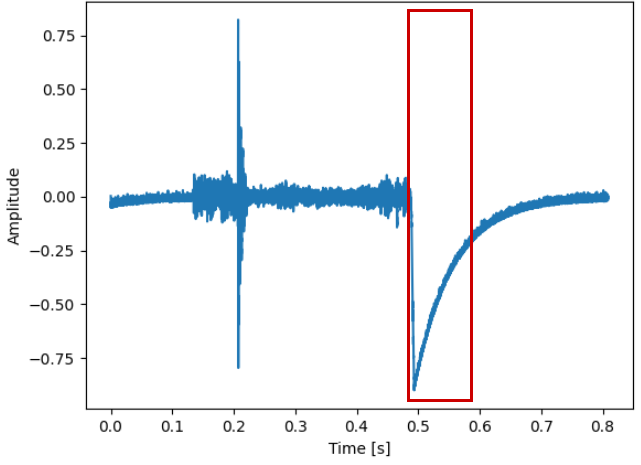
\includegraphics[width = 0.63\textwidth]{obrazky-figures/ptt.png}
        \caption{Push-to-talk signal in audio recording.}
        \label{fig:ptt}
    \end{figure}

\newpage    
\subsection{Push-To-Talk and Air Traffic Control}\label{PTTinATC}

When a~pilot activates their PTT switch to transmit a~message, it can serve as an indication to the VAD system that a~new speaker has started speaking. This information can then be used to identify different speakers and help ATC to reduce confusion and interference on the frequency. Push-to-talk switches can fail, which could disable transmitting messages.

The pressed PTT button or switch activates the aircraft's radio transmitter, which allows the pilot to transmit their message to the ATC tower or other aircraft. Simultaneously, the aircraft's receiver is muted, which prevents the incoming transmission from being heard by the pilot. 

When the button is released, the transmitter is turned off, and the receiver is unmuted, which allows further communication. 


In aviation communication systems, PTT is usually activated through a~button or switch located on the control wheel or yoke of the aircraft. This allows the pilot to keep their hands on the controls while transmitting their message. Some aircraft may also have additional PTT buttons or switches located on the instrument panel or elsewhere in the cockpit for use by other crew members.



%When the PTT button or switch is pressed, it activates the aircraft's radio transmitter, allowing the pilot to transmit their message to the air traffic control tower or other aircraft. 

%At the same time, the aircraft's receiver is muted, preventing incoming transmissions from being heard by the pilot. When the PTT button or switch is released, the transmitter is turned off, and the receiver is unmuted, allowing the pilot to hear incoming transmissions.

%=========================================================================

\chapter{Used Datasets and Data Augmentation}\label{Data}

    An overview of signal processing techniques and a~description of the ATCO2\footnote{see \href{https://www.atco2.org/}{{\fontfamily{cmtt}\selectfont https://www.atco2.org/}}} project can both be found in this chapter. It will be discussed in more detail later how the dataset for Push-To-Talk was assembled and labelled. 

    Data preparation for neural network training is a~challenging process. An unbalanced dataset, inaccurate labels, or poor-quality data are a~few of the factors that might make neural network training fail. Providing a~precise dataset is needed to avoid overfitting or underfitting the neural network and to obtain desired results.
    
    
\section{ATCO2 Dataset}\label{Dataset}

    \textit{ATCO2} project\footnote{see \href{https://www.atco2.org/}{{\fontfamily{cmtt}\selectfont https://www.atco2.org/}}} concentrates on developing a~platform where voice communication can be collected, organized and pre-processed \cite{zeytinoglu2008voice}. The data is collected through very high-frequency radio receivers that are owned by a~community of volunteers.
    
    \vspace{0.2cm}
    
    The data processing pipeline consists of:
    \begin{enumerate}
        \item speech pre-processing tools such as segmentation or volume adjustment
        \item diarization which is used to split audio by speakers
        \item automatic speech recognition
        \item English language detection
        \item speaker role detection, which can be ATCO or pilot
        \item labelling of call signs, commands and values
    \end{enumerate}

    This pipeline was used to produce the dataset that was provided for this thesis. The provided dataset contains four hours of ATC speech with manual transcripts.
    The dataset was built for the development and evaluation of \textit{Automatic Speech Recognition} and \textit{Natural Language Processing} for the ATC domain. The audio files in this dataset are sampled at 16,000kHz. 


    \newpage
    The structure of the dataset is explained in the following figure:

    \begin{figure}[ht!]
        \dirtree{%
            .1 ATCO\_TEST\_SET\_4H.
            .2 release.
            .3 LISTS.
            .4 accepted.list.
            .3 DATA.
            .4 LSGS\_SION\_Ground\_Control\_121\_7MHz\_20210503\_122624.wav.
            .4 LSGS\_SION\_Ground\_Control\_121\_7MHz\_20210503\_122624.segm.
            .4 LSGS\_SION\_Ground\_Control\_121\_7MHz\_20210503\_122624.cnet.
            .4 ....
            .3 DATA\_nonEN.
            .4 ....
        }
    \caption{Tree structure of provided data folder.}
    \label{fig:ATCO_Structure}
    \end{figure}
    

    As it is shown in the example of files in the folder (figure \ref{fig:ATCO_Structure}) the most important files in this dataset are wav files.
    
    Other important files are \texttt{CNET} files and \texttt{SEGM} files. \texttt{CNET} files contain annotation for every word that was detected in the audio using the \textit{Kaldi confusion network} which is an automatic transcript, and \texttt{SEGM} files contain speech segments.  Nearly every audio was annotated, and approximately 66\% of audio was accepted as correctly annotated by the human re-checker. 

\section{Data Pre-Processing}\label{Dataset NN}

    Signals are converted into spectrograms and then fed into a~neural network. Spectrograms are visual representations of signal strength, or ``loudness'' over a~time period and frequency. High energy levels and low energy levels are easy to distinguish visually. To enhance spectrogram features, it is conventional to apply MelBank filters \cite{Leitner2019AudioRU}. Mel spectrogram is created by converting the spectrum into Mel Scale. 
    \begin{itemize}
    	\item a~spectrum is created by transforming the signal from time domain\footnote{Continuous signal into discrete frequencies.} to the frequency domain using the Fourier Transform mathematical formula \cite{heckbert1995fourier}:
     
            \begin{equation}\label{FT}
    	   F(\omega)=\int_{-\infty}^{\infty} f(x) \cdot e^{-i \omega x} d x
            \end{equation}
    	
    	\item Mel Scale is a~non-linear representation of human perception of sound. The frequencies are converted using a~formula:
            \begin{equation}\label{MS}
                m = 2595 \cdot \log _{10}\left(1+\frac{f}{700}\right)
             \end{equation}
    
        where $m$ represents Mel and $f$ represents frequency \cite{o1987speech}.
    \end{itemize}	

    \newpage

    The neural network will get a~glimpse of how humans perceive sound by transforming the original signal into a~Mel Spectrogram. 
    The process of generating a~Mel Spectrogram is shown in figure \ref{fig:SIGNALMELPIPELINE}.

    \begin{figure}[ht!]
        \centering
        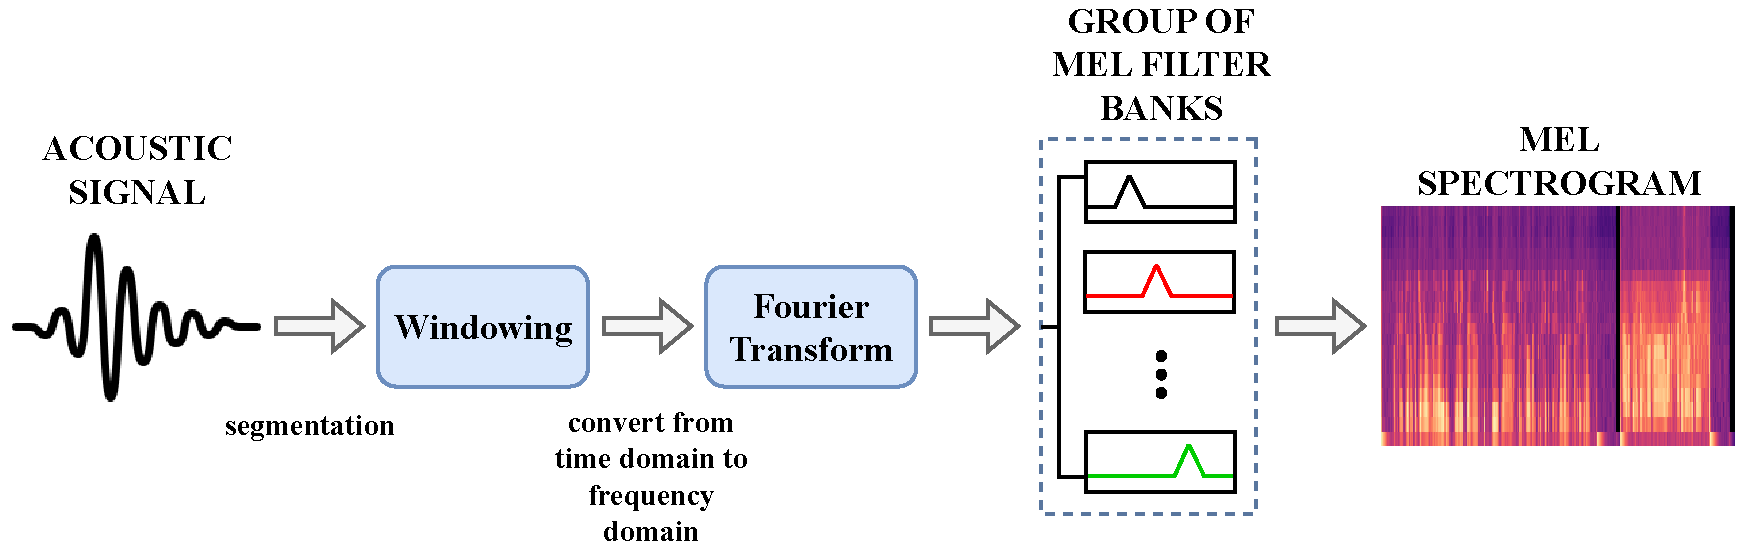
\includegraphics[width = \textwidth]{obrazky-figures/mel_pipeline.pdf}
        \caption{Pipeline to generate Mel spectrogram.}
        \label{fig:SIGNALMELPIPELINE}
    \end{figure}

    Mel Spectrograms were generated differently for each implementation (table \ref{tab:comparsionFNNGPVAD_mel}).

    \begin{table}[ht!]
        \centering
        \begin{tabular}{|c|c|c|c|c|c|c|} \hline
            & \textbf{Window (ms)} & \textbf{Overlap (ms)} & \textbf{Mels} & \textbf{Window Function} & \textbf{Post-Log} \\  \hline
            \textbf{ENN} & 25 & 10 & 20 & Hamming & no\\ \hline
            \textbf{GPVAD} & 40 & 20 & 64 & Hamming & yes \\\hline
        \end{tabular}
        \caption{Table shows key differences in pre-processing signal.}
        \label{tab:comparsionFNNGPVAD_mel}
    \end{table}

     Experimental Neural Networks (ENN) window duration and overlap duration are shorter compared to GPVAD's \cite{Dinkel2020, Dinkel2021} parameters (table \ref{tab:comparsionFNNGPVAD_disadv}). GPVAD's log Mel Spectrogram can present the characteristics in the low- and high-frequency regions with greater detail than the non-logarithmized Mel Spectrogram \cite{Seo_Kim_Kim_2022}.

    \begin{table}[ht!]
        \centering
        \begin{tabular}{|c|c|c|} \hline
            & \textbf{Detecting Short-Lived Features} & \textbf{Better Frequency Resolution} \\  \hline
            \textbf{ENN} & yes & no \\ \hline
            \textbf{GPVAD} & no & yes\\ \hline
        \end{tabular}
        \caption{Table shows key differences in pre-processing signal.}
        \label{tab:comparsionFNNGPVAD_disadv}
    \end{table}

    It is hard to determine which parameters are better due to opposition advantages and disadvantages \cite{BENZEGHIBA2007763}. Each of the pre-processed signals is shown in figures \ref{fig:Melspec_FNN} and \ref{fig:Melspec_GPVAD}. Signal pre-processing is a~crucial part of preparing the data to feed the neural network. Mel Spectrograms have been shown to be very beneficial. 

    \newpage
    
    Using the MFCC\footnote{Mel Frequency Cepstral Coefficients.} as input is another strategy. MFCC is an extension of the Mel Spectrogram. The Logarithm of Mel spectrogram magnitudes undergoes the process of Discrete Cosine Transform and coefficients are created \cite{MFCCs}. 

    \begin{figure}[ht!]
        \centering
        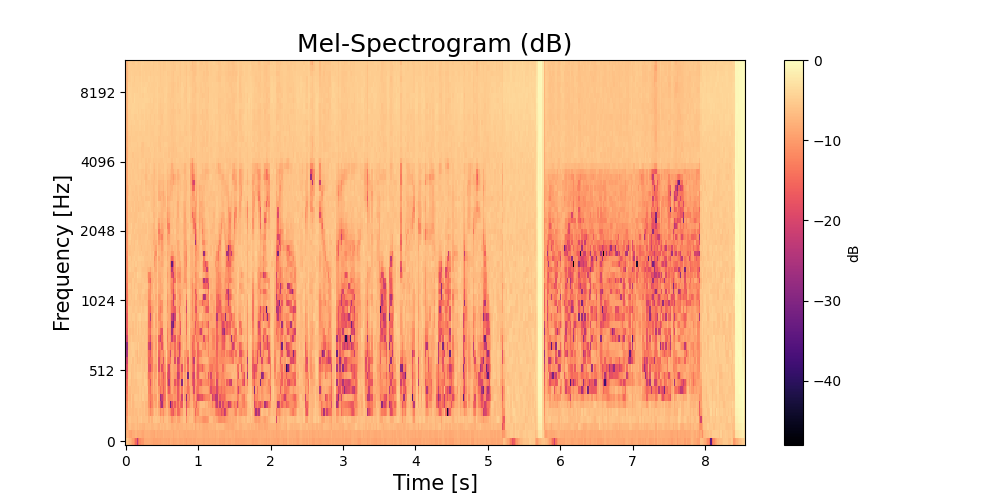
\includegraphics[width = \textwidth]{obrazky-figures/GPVAD.png}
        \caption{Mel spectrogram input for GPVAD implementation.}
        \label{fig:Melspec_GPVAD}
    \end{figure}

    \begin{figure}[ht!]
        \centering
        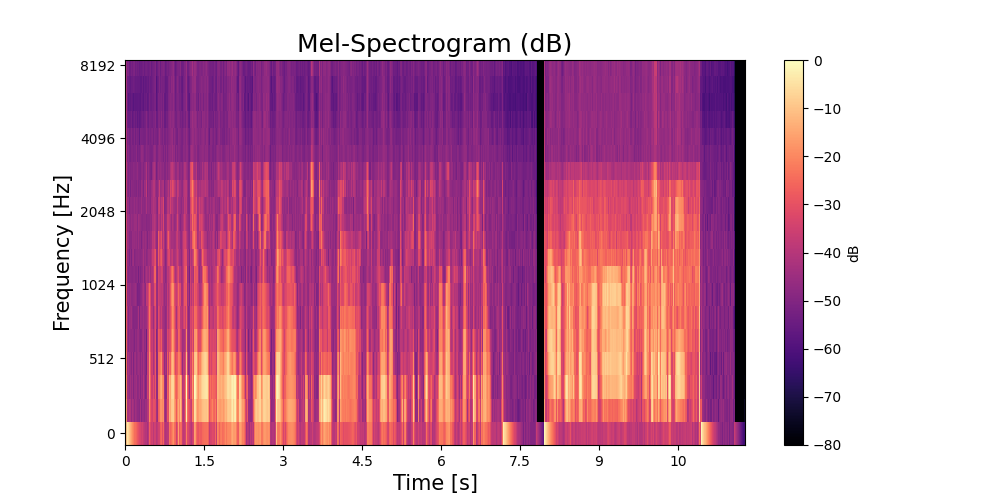
\includegraphics[width = \textwidth]{obrazky-figures/FNN.png}
        \caption{Mel spectrogram input for ENN implementation.}
        \label{fig:Melspec_FNN}
    \end{figure}

\newpage

\section{Dataset for Push-To-Talk}\label{Dataset for PTT}

    a~balanced dataset is necessary for effective neural network training, as was described in the section \ref{Augmentation}. ATCO2 provides audio files which contain recordings that vary in duration. Almost every audio has a~minimum of one push-to-talk (PTT) signal. 
    
    As discussed in section \ref{PTT}, the push-to-talk signal is represented by temporarily muting the transmitter. Push-to-talk is most of the time easily identified in the recordings (see figure~\ref{fig:sigPTT}). 


    \begin{figure}[ht!]
        \centering
        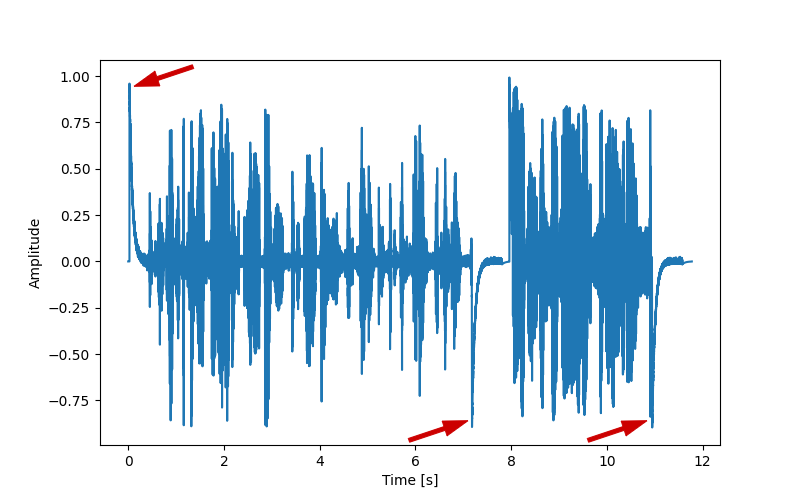
\includegraphics[width = 0.9\textwidth]{obrazky-figures/signalwithPTT.png}
        \caption{Image of audio with three push-to-talk events highlighted by the red arrows.}
        \label{fig:sigPTT}
    \end{figure}


    In this dataset, the PTT signal could be classified into three categories (figure \ref{fig:typesPTT}):

    \begin{itemize}
        \item \textbf{A clear PTT signal} has the biggest representation in the dataset. PTT of this kind is easily recognized by algorithms or by humans. 
        \item The second most represented category is \textbf{noisy PTT signals}.
        It makes sense that noise-free recordings are frequently challenging to get through air traffic control. Usually, there is excessive noise in the audio, especially on the pilot side. PTT events can be detected despite background noise by using filters that reduce noisy backgrounds. 
        \item The last category represents \textbf{double-pressed or multiple-time pressed} PTT signals. This can occur by mistake or by certain configurations of the technology.
    \end{itemize}


    a~logical distribution between non-PTT and PTT events is necessary when training a~neural network to detect push-to-talk signals. The audio's speech and non-speaking segments can both be classified as non-PTT events. Using the~PEEK algorithm (see~\ref{Labeling}) audio segments were extracted and one by one manually checked. These segments were used in combination with segments that did not contain PTT events. By randomly selecting from each group, a~dataset was created.

    In the process of creating the dataset, localised push-to-talk events were produced from each audio in the ATCO2 dataset by the PEEK algorithm. Each detected event was manually checked and evaluated if it should be stored in the dataset. This way, over, 3500 push-to-talk events were checked and accepted by hand. 

    In summary, the process of creating a~dataset that should be used in order to train a~model to detect PTT events was quite challenging. In order to reduce False Alarms, it was important to include in the dataset recordings which did not contain any PTT signal.



    \begin{figure}[ht!]
        \centering
        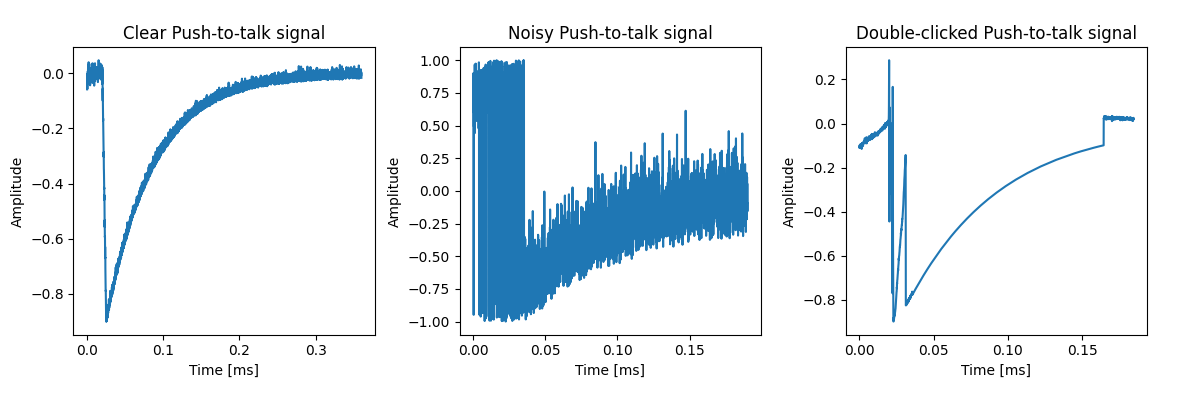
\includegraphics[width = \textwidth]{obrazky-figures/TypesOfPTT.png}
        \caption{Types of PTT signal.}
        \label{fig:typesPTT}
    \end{figure}

    The dataset is containing two types of recordings. The first type represents audio files with no push-to-talk event. The second type contains recordings in which at least one push-to-talk event occurred. These recordings contain from one to five push-to-talk events. 


\section{Data Labelling}\label{Labeling}

    This section can be divided into two parts: labelling voice activity (see \ref{LabelVAD}) and push-to-talk (see \ref{LabelPTT}). 
    
    Labelling data is the most challenging part of creating a~dataset. To supervise the training of the neural network, high-quality labels are necessary. The main goal is to create labels with a~very low error rate. The process of creating labels for voice activity was easier in comparison with labels for push-to-talk. 


    \subsection{Labelling Voice Activity}\label{LabelVAD}

        Annotations for voice activity detection were included in the ATCO2 dataset. As stated in section \ref{Dataset} \texttt{CNET} files contained transcriptions to text for each word in the communication. The transcriptions were generated by \textit{Hybrid Automatic Speech Recognition}. Labels from these files were used while creating labels for the ENN neural network training, considering more precise speech segments. \texttt{SEGM} files contain segments of speech which are more suitable for final comparison between different approaches.

        Labels were generated from processing \texttt{CNET} files, which contain timestamps for each word. Each frame in Mel Spectrum was a~label assigned. Missing segments from files were substituted by placing non-speech labels in their place. 
        \newpage
        In figure \ref{fig:CNETVSSEGM} the difference between \texttt{CNET} files and \texttt{SEGM} files is shown. 

        \begin{figure}[ht!]
            \centering
            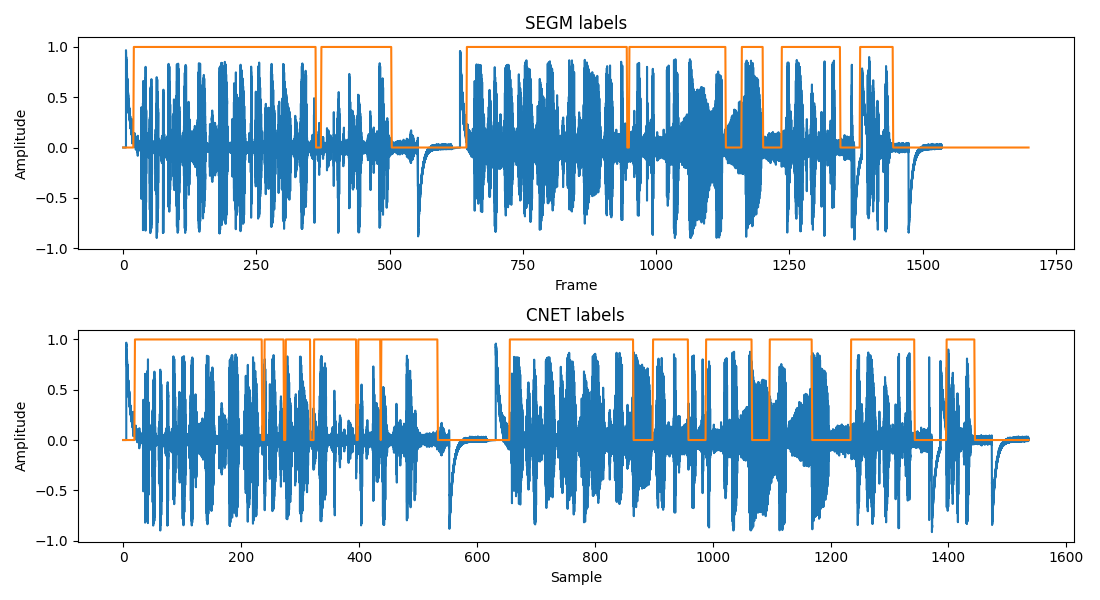
\includegraphics[width = \textwidth]{obrazky-figures/cnetVSsegm.png}
            \caption{Comparison between two available labels from files. Label one represents speech and label zero represents non-speech.}
            \label{fig:CNETVSSEGM}
        \end{figure}

        Labels for GPVAD implementation were generated from the output of the pre-trained model. This will be further explained in chapter \ref{Implementation}. 
        

    \subsection{Labelling Push-To-Talk}\label{LabelPTT}

    The ATCO2 dataset does not contain PTT labels. It would be possible to go over each audio in the dataset and label it in some programs like Audacity, but this process would be very time-consuming. To automatize the process of labelling, various approaches were tried.
    Every one of them was concentrating on sudden changes in signal energy. It is important to mention that the duration of the PTT varies. To generalize the PTT event, a~threshold of 100 ms was selected. This threshold represents a~minimal duration of the event. 

    In the first attempt, the power of each frame was considered. By analysing the values of the spectrogram, the potential start of the peak was selected, and its neighbourhood was examined. The basic idea of this approach was to examine the sudden drop and smooth increase of signal in an adjacent area to a~potential peak. 
    \newpage

    \vspace{0.5cm}
    \SetKwComment{Comment}{/* }{ */}
    \begin{algorithm}
    \caption{PTT detection algorithm based on analysing spectrogram.}\label{alg:one}
        \KwIn{Signal}
        \KwOut{Labels for PTT}
        
        \vspace{0.3cm}
        \SetNlSkip{-2.0em}
        \SetNlSty{}{}{:}
        \Indp
        \Indp  
        examination = False;\\
        final evaluation = False;
        
        \ForEach{frame in audio}{
            \If{lower energy in the frame}{
                potential frame selected;\\
                examination = True;
            }
        
            \If{examination}{
                examine the current frame for a~smooth increase \\
                \If{examinating for x frames}{ 
                    examination = False;\\
                    final evaluation = True;
                }
            }
        
            \If{final evaluation}{
                check sudden drop; \\
                check smooth increase;\\
                check the power of the potential frame;\\
                \If{every check succesful}{
                    add a~potential frame to the PTT array;
                }
                final evaluation = False;
            }
        }
        
        \ForEach{element in PTT array}{
        previous two frames, the selected frame, and seven following frames are labelled as PTT event;
        }
    
    \end{algorithm}


    This method seem promising at first because it could detect peaks with certain negative amplitude. Despite that, its overall performance had shown to be really poor. It was not generic enough to capture each PTT event and label it correctly because of the specific values. After examination, most of the PTT events were missed. On the other hand, the percentage of false alarms was close to zero, This algorithm was not sufficient to use as an automatic label method. 

    
    After bad results and a~realisation that the push-to-talk event is not only the negative amplitude, the strategy changed. The second attempt was similar to the first attempt. It was still necessary to revolve around changes in amplitude. The signal is examined for both positive and negative peaks. Using Python library functions \texttt{find\_peaks}\footnote{see \href{https://docs.scipy.org/doc/scipy/reference/generated/scipy.signal.find_peaks.html}{{\fontfamily{cmtt}\selectfont https://docs.scipy.org/doc/scipy/reference/generated/scipy.signal.find\_peaks.html}}} and \texttt{find\_peaks\_cwt}\footnote{see \href{https://docs.scipy.org/doc/scipy/reference/generated/scipy.signal.find_peaks_cwt.html}{{\fontfamily{cmtt}\selectfont https://docs.scipy.org/doc/scipy/reference/generated/scipy.signal.find\_peaks\_cwt.html}}}  to find peaks was unsuccessful. Peaks were not correctly recognised. The outcomes were not applicable to the final detection. 

    One appeared more promising than the others after multiple attempts of finding satisfactory peak detection algorithms. Local maxima might be easily found throughout the signal by using a~peak detection method called \textit{peakdet}\footnote{see \href{http://billauer.co.il/blog/2009/01/peakdet-matlab-octave/}{{\fontfamily{cmtt}\selectfont http://billauer.co.il/blog/2009/01/peakdet-matlab-octave/}}} converted from Matlab to Python by Eli Billauer \cite{peakdet}. As the delta value $0.2$ was chosen as it seemed the most optimal value. 

    The push-to-talk event starts with high negative or positive amplitude, after which the upcoming $100 ms$ does not flip over zero. The position of the peak is usually at the beginning of the corresponding number of frames. 

    Conditions for elimination were used once the peaks had been retrieved. When the signal did not flip over zero for at least 100 milliseconds and the peak was a~local extreme in the adjacent area, it can be classified as a~PTT event. The additional search for local extreme in the neighbourhood\footnote{The interval starts at the first flip over zero sample before the peak. It ends at the last sample after the peak before flipping over zero.} excludes peaks that were not excluded in the duration test. This test is especially useful for double-pressed PTT signals.  
    
    The PTT labelling was greatly automated thanks to this algorithm. Both ENN and GPVAD implementations rely on labels produced by this technique. 
        
    \vspace{0.5cm}
    \SetKwComment{Comment}{/* }{ */}
    \begin{algorithm}
    \caption{PTT detection algorithm (PEEK) based on peak detection in a~signal.}\label{alg:two}
      \KwIn{Signal}
      \KwOut{Labels for PTT}
        \vspace{0.3cm}
        \SetNlSkip{-2.0em}
        \SetNlSty{}{}{:}
        \Indp
        \Indp 
        positive peaks, negative peaks = peakdet (signal);

        \ForEach{peak in negative peaks}{
            \If{peak is negative for at least 100 ms}{
                keep;
            }
            \If{peak is local extreme in its negative neighbourhood}{
                keep;
            }
        }
        \ForEach{peak in positive peaks}{
            \If{peak is positive for at least 100 ms}{
                keep;
            }
            \If{peak is local extreme in its positive neighbourhood}{
                keep;
            }
        }
    \end{algorithm}
    \footnotetext{\href{http://billauer.co.il/blog/2009/01/peakdet-matlab-octave/}{{\fontfamily{cmtt}\selectfont http://billauer.co.il/blog/2009/01/peakdet-matlab-octave/}}}
    \vspace{0.3cm}

    The final comparison between these two approaches was evaluated on 1000 recordings from the PTT dataset (see \ref{Dataset for PTT}) which contained various numbers of PTT events.
    \newpage
    Table \ref{tab:comparisionapproaches} shows the difference in causing false alarms and missed hits with each approach. 

    \vspace{0.2cm}

    \begin{table}[ht!]
        \centering
        \begin{tabular}{|c|c|c|c|} \hline
            & \textbf{Missed Push-Po-Talk (\%)} & \textbf{False Alarms} & \textbf{Accuracy (\%)} \\ \hline
            \textbf{Algorithm \ref{alg:one}} & 81.30 & 8 & 18.70\\ \hline
            \textbf{Algorithm \ref{alg:two}} & 0.30 & 0 & 99.70\\ \hline
        \end{tabular}
        \caption{In the dataset, there were 988 PTT events.}
        \label{tab:comparisionapproaches}
    \end{table}

    \vspace{0.2cm}

    As is shown in table \ref{tab:comparisionapproaches} the second algorithm is far better than the first one. It correctly identified most of the PTT events and didn't cause any false alarms. On the other hand, the first algorithm performed poorly in detecting PTT events and caused 8 false alarms. The second algorithm's performance is more than sufficient for generating labels automatically. The dataset consisted of manually checked push-to-talk events. 

    The length of the PTT event varies. This is because some of the frames that are considered to have a~PTT peak in them could have this peak at the end of the frame, which could cause mislabelling. PTT event lasts for approximately 100ms. This is due to prevent another mislabelling of silence for the PTT event. This topic and experiments with labelling will be further explained in chapter \ref{Implementation}. 

    PTT labels generated from the second algorithm are shown in figure \ref{fig:pttlabels}.
    
        \begin{figure}[ht!]
            \centering
            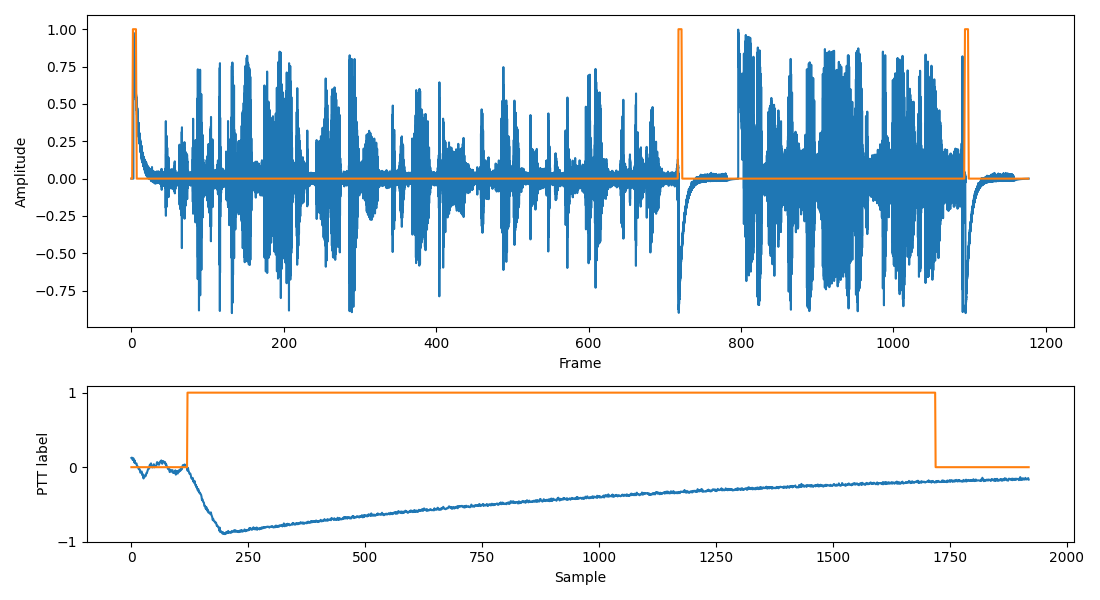
\includegraphics[width = 0.9\textwidth]{obrazky-figures/PTTlabel.png}
            \caption{The upper graph shows a~whole image with three PTT events. The bottom graph is zoomed to one of the labelled push-to-talk events. }
            \label{fig:pttlabels}
        \end{figure}

    During training the neural network on multitask detection, it is important that labels do not cause a~conflict. The push-to-talk event can be only possible when the non-speech frame is present in the second class. Training on datasets with wrong labels would lead to a~deterioration of accuracy.

    \newpage
    
    \section{Augmentation Techniques}\label{Augmentation}

    Employing augmentation can boost neural networks' capacity for generalisation. Augmentation is a~popular preprocessing technique used in the neural network training process. The dataset becomes more robust and varied, which can aid in the training process and improve the classification accuracy of new incoming data. The application of time-domain modification is the method used most frequently to enhance signal data \cite{xu2022mixing}. Some of the most common techniques are \cite{DBLP:journals/corr/SalamonB16}:
    
    \begin{itemize}
        \item \textbf{Time Stretching} is a~method when the audio is slowed down or sped up while keeping the pitch unchanged. 
        \item \textbf{Window Slicing} method refers to randomly selecting a~time range which is downsampled or upsampled. Other time ranges remain untouched.
        \item \textbf{Magnitude Slicing} refers to a~method during which the magnitude of the signal is modified. It is done by multiplying the original magnitude of the signal at a~certain position with another selected magnitude.
        \item \textbf{Noise Injection} is another very commonly used method in signal augmentation. It is done by adding noise to certain signal parts. The labels for these parts remain unchanged.
    \end{itemize}

    Other techniques such as normalising the signal or noise filtering can improve the quality of the dataset. Figure \ref{fig:augmentationtechniques} shows various signal changes after applying some augmentation techniques.

    
    \begin{figure}[ht!]
        \centering
        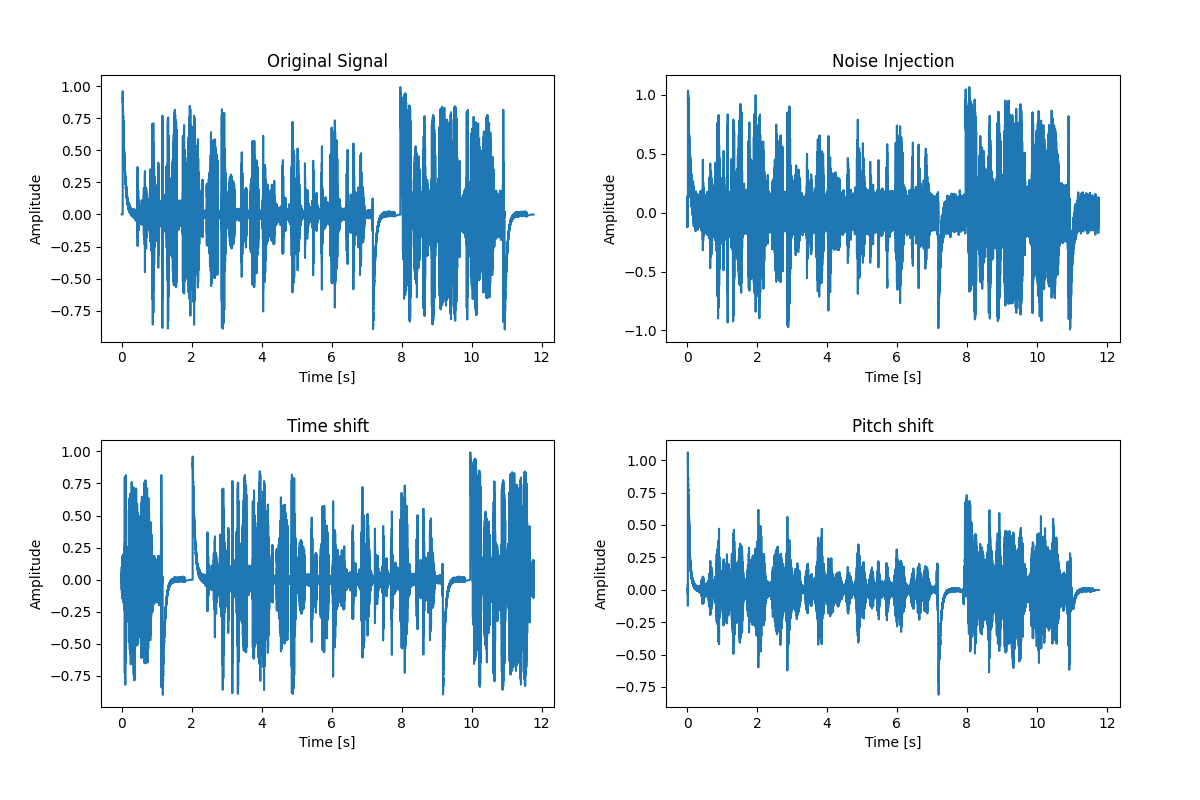
\includegraphics[width = 0.95\textwidth]{obrazky-figures/augmentation.png}
        \caption{Augmentation techniques.}
        \label{fig:augmentationtechniques}
    \end{figure}

    \newpage

    This chapter provided an overview of the used datasets in this implementation. The main source of audio files was the dataset by the ATCO2 project.

    The ATCO2 dataset contains hours of air traffic communication. Ground truth labels for speech detection were provided in the files of the dataset and used to generate labels for training the models.
    
    The dataset did not contain labels for push-to-talk so an algorithm was proposed. The first algorithm was not efficient enough to detect the push-to-talk events. Another approach was proposed and used for final PTT detection. The PEEK algorithm can correctly detect push-to-talk events even in noisy environments. 

    Finally, augmentation techniques are introduced and explained. 


    
    
%=========================================================================

\chapter{Proposed solution and Implementation}\label{Implementation}

    This chapter will provide an overview of the thesis's goal, implementation pipelines, used technologies, and selected architectures for neural networks.

\section{Definition of the Task}

    The primary goal of this thesis is to construct a~neural network that is capable of both simultaneous predictions of speech and non-speech segments, as well as detection of the PTT event. 
    The process of getting predictions for two or more tasks from a~neural network is called multitask learning \cite{DBLP:journals/corr/abs-2009-09796}. 

    The capacity of doing the task with a~smaller number of models is one of this strategy's main advantages. The ability to make predictions while multitasking comes naturally to humans. Analysing an object and determining its characteristics simultaneously is done without much thought.
    Such things as predicting two outcomes together can be learnt by neural networks.
    The learning process could be enhanced due to this strategy, considering training with more context.
    It is quite simple, the more data provided, the better generalization and learning of the neural network.
    But there are also downsides to this strategy. It could be challenging to simultaneously train a~neural network for two tasks if the objectives are incompatible. 

    \begin{figure}[ht!]
        \centering
        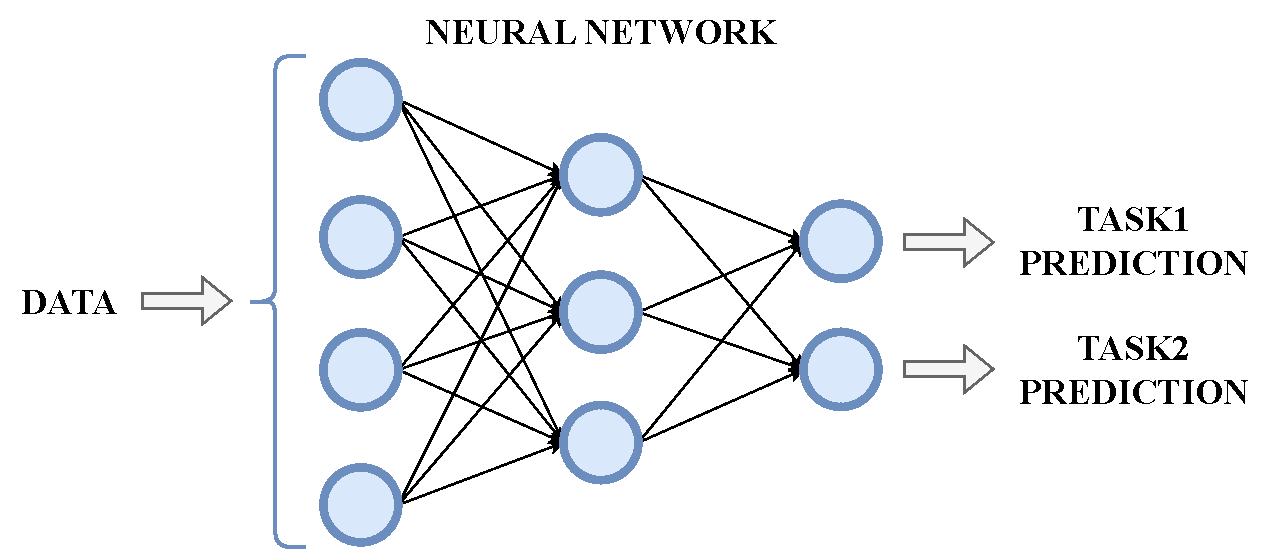
\includegraphics[width = 0.8\textwidth]{obrazky-figures/MTL.pdf}
        \caption{Abstract visual example of a~multitask neural network.}
        \label{fig:MTL}
    \end{figure}
    
    In the next section \ref{Architectures} it will be talked about creating such architecture and the adaptation process of existing implementations will be explained. 
        
\section{Used Technologies}

    The program is implemented in the programming language Python. Python has various libraries which can be used in the process of training and validating the neural network. This program is using library \texttt{PyTorch}\footnote{see \href{https://pytorch.org/}{{\fontfamily{cmtt}\selectfont https://pytorch.org/}}} which is commonly used in this field. It contains various methods that lead to efficient work with neural networks.

    For audio processing, the most frequently used libraries were \texttt{librosa}\footnote{see \href{https://librosa.org/doc/latest/index.html}{{\fontfamily{cmtt}\selectfont https://librosa.org/doc/latest/index.html}}}, \texttt{numpy}\footnote{see \href{https://numpy.org/}{{\fontfamily{cmtt}\selectfont https://numpy.org/}}} and \texttt{scipy}\footnote{see \href{https://scipy.org/}{{\fontfamily{cmtt}\selectfont https://scipy.org/}}}. Each one contains various functions which help to work with the audio. 
    

\section{Selected Architectures}\label{Architectures}

    The architecture of each neural network is presented and discussed in this section. 
    Each neural network consists of connected layers, and each time data passes through a~layer, an activation function is applied. This process was explained in chapter \ref{ANN}.
    How supervised training operates is demonstrated in figure \ref{fig:pipeline}. There are several steps in the training process. 
    To sum all it up, pre-processed data are fed into a~neural network and the model modifies its weights based on the difference between ground truth and predicted output. 


    \begin{figure}[ht!]
        \centering
        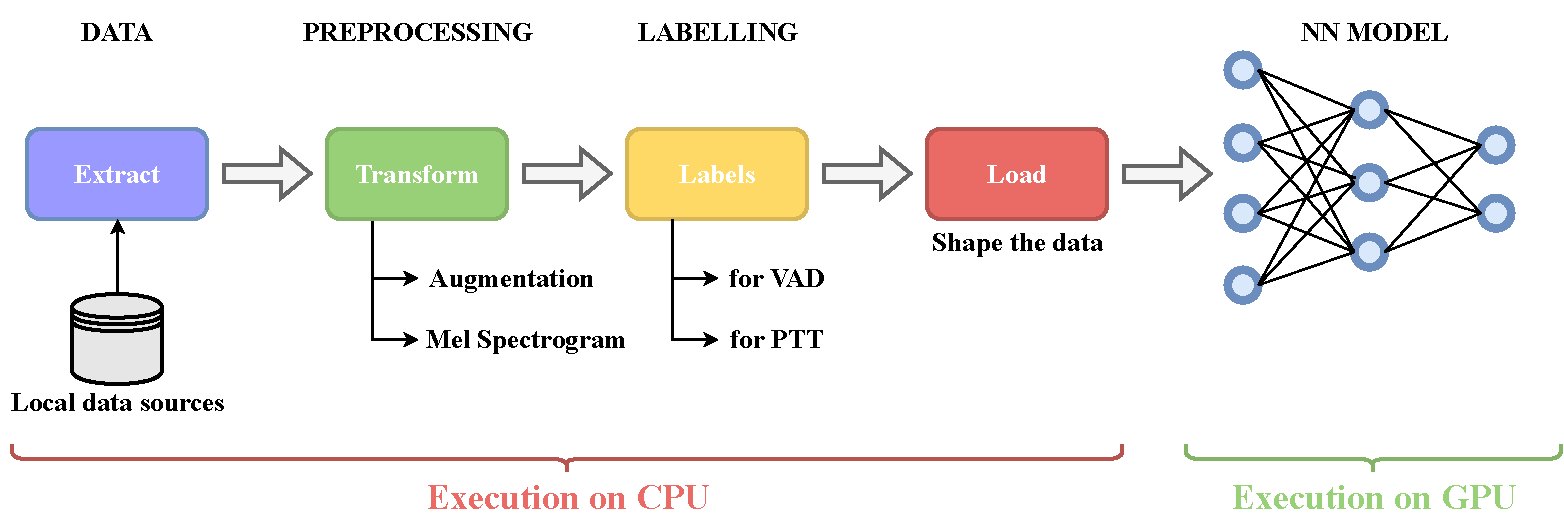
\includegraphics[width = \textwidth]{obrazky-figures/pipeline.pdf}
        \caption{Abstract visual example of a~multitask neural network.}
        \label{fig:pipeline}
    \end{figure}

    The first experimental neural network is a~basic feed-forward neural network with two hidden layers. To further understand the neural network, this step was necessary. 
    
    

\subsubsection{Proposed Architectures for Initial Experiments}\label{ENNarch}

    The implementation was centred on experimenting with various neural network designs. 
    Architecture refers to the design of the model. A~model can be represented in a~number of units and their pattern connection.
    
    To get acquainted with the neural networks, the first proposed architecture was rather simple. It was a~basic feed-forward model.
    This model was made up of two hidden layers. 
    
    As seen in figure \ref{fig:NN}, the model was quite basic, which was convenient for grasping knowledge about neural networks.

    \begin{figure}[ht!]
        \centering
        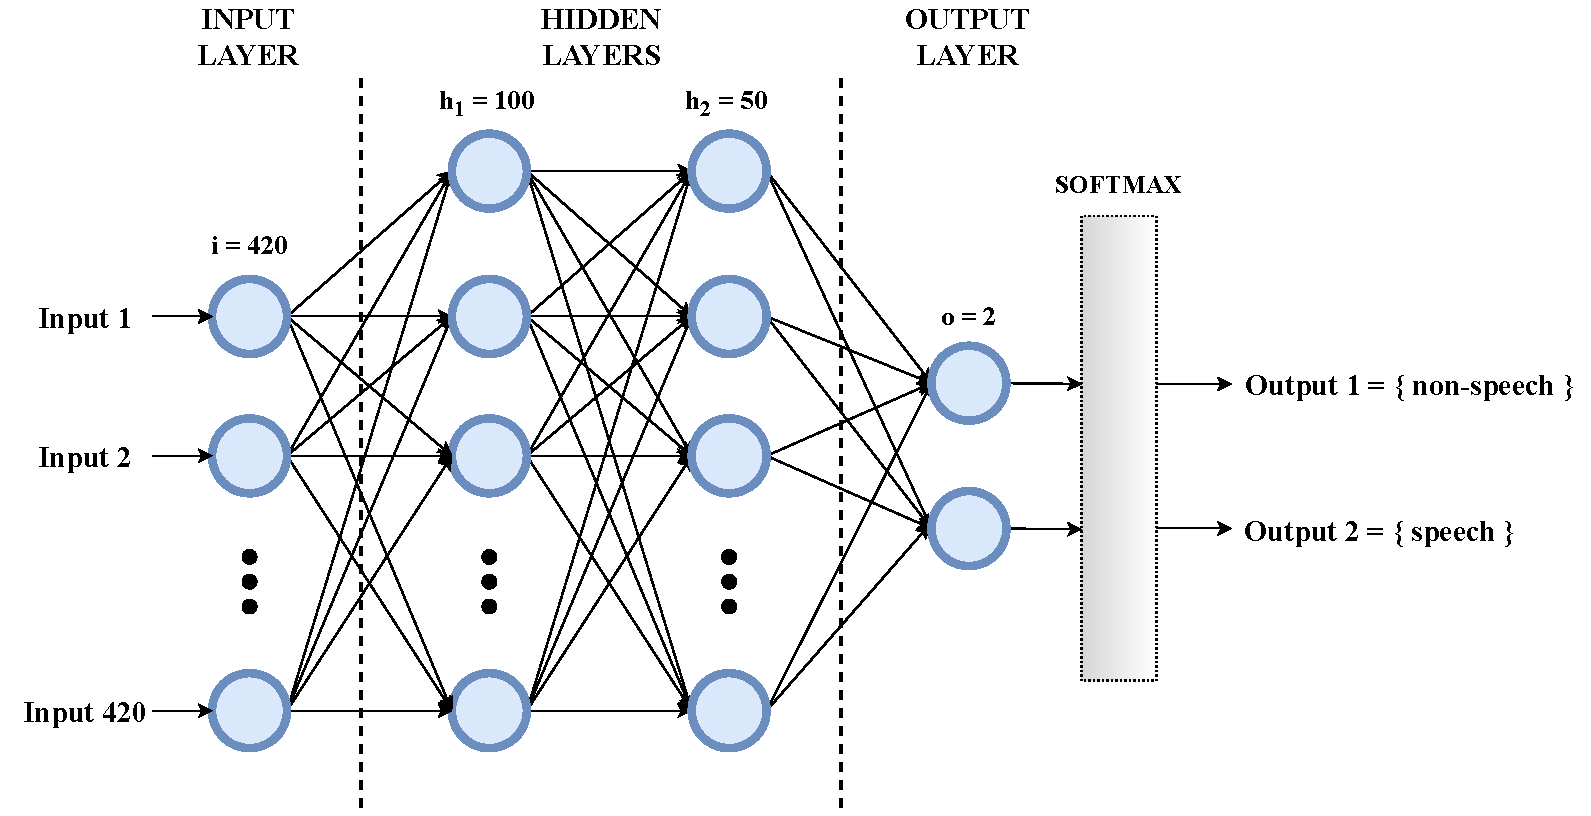
\includegraphics[width = \textwidth]{obrazky-figures/NN1.pdf}
        \caption{Architecture of a~simple neural network}
        \label{fig:NN}
    \end{figure}

    The model was trained only to distinguish between speech and non-speech frames before constructing a~proper algorithm for push-to-talk recognition. A~collection of frames represents the input to this neural network. Each frame generated during the Mel Spectrogram creation process represents a~set of frequencies. Frames could represent different meanings in different locations. That is why it was necessary to provide further context. Adjacent frames have been joined together to produce more informative surrounds. As a~result, input to the neural network is a~sequence of 21 frames ($210$ ms) rather than a~single frame ($10$ ms). This is also due to the fact that one phoneme is at least $100$ ms long \ref{VAD}. A~group of frames with 20 frequencies each after removing one dimension created an input array of length 420 (figure \ref{fig:NN}).

    ReLu was used as an activation function. It was chosen because it is one of the most popular and used activation functions due to its non-linearity and robustness to vanishing gradients. It is also computationally undemanding. On the final layer, the Softmax function was applied. The result was a~probability for each class. 
    
    % proposal of MTL architecture
    After implementing the PEEK algorithm, multitasking was added to the neural network. It has the same architecture as the previous model, but with an additional output layer for PTT detection (figure \ref{fig:NN}). 
    
    % example of architectures using convolutional models
    To further understand various types of neural networks, another model was created. Because the neural network is basically fed by visual representation\footnote{Spectrogram.} of audio, it is clear that adding convolutional layers could improve performance. 

    

    The second experimental model has two convolutional layers. The input shape changed as well. The input was not flattened as it was in the FNN approach but kept in a~two-dimensional shape. This means that now neural network works with image-like input. Input is a~two-dimensional array of size $21\times20$. An explanation of this choice was explained earlier in the text. This neural network is shown in figure \ref{fig:CNN2D}. 

    \begin{figure}[ht!]
        \centering
        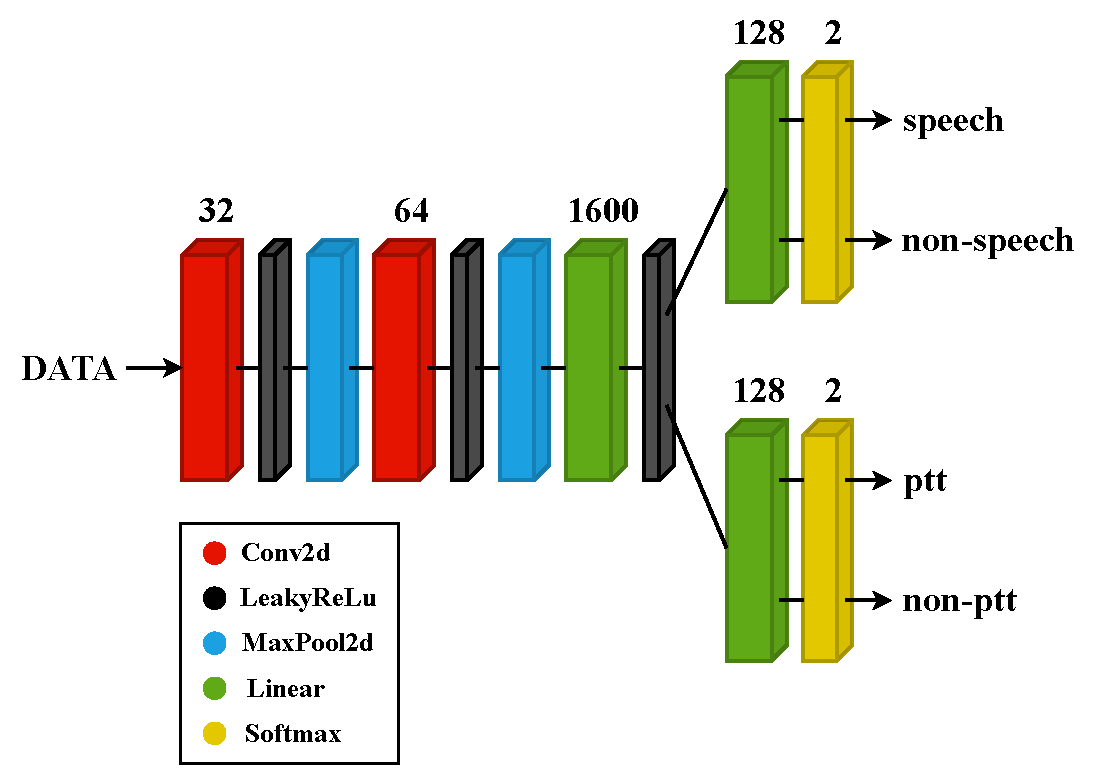
\includegraphics[width = \textwidth]{obrazky-figures/CNN2D.pdf}
        \caption{Architecture of a~convolutional neural network with two-dimensional input.}
        \label{fig:CNN2D}
    \end{figure}

    The first convolutional layers contain 32 convolutional filters and the second layer contains 64 filters.
    Between those two layers, the activation function ReLu is applied and the max-pooling layer is provided. Max pooling is one type of pooling operation which takes responsibility for highlighting the significant features as well as reducing spatial dimensions.

    The creation of model architectures was done by combining learnt knowledge, experimenting and testing the NN models. Proposed models are quite simple and not too complex to learn. Simple models can often outperform complex models. 
    The training process and experiments with those architectures will be further explained in chapter \ref{Experiments}. Various architectures can change the accuracy of detecting voice activity and push-to-talk events. 


\subsubsection{Adaptation of GPVAD}\label{GPVADarch}

    Because neural networks need tons of data to properly learn and generalize to new data, it is conventional to use pre-trained models. It is possible to use some knowledge of previously trained models. The choice of those neural networks depends only on the specific problem. In this implementation, the GPVAD approach was adapted \cite{Dinkel2020, Dinkel2021}.   

    GPVAD\footnote{General purpose voice activity detection.} uses weak labelled supervision on clip level, which can outperform strongly supervised VAD during the evaluation of real-world data or noisy datasets. 
    
    GPVAD's performance is not significantly better than traditional approaches\footnote{For example models which used Hidden Markov Model as frame-level labels.}, but trained models do a~good job of detecting speech in noisy environments. This characteristic is very useful in terms of detecting speech in air traffic communication, which is an environment with high background noise. The teacher-student approach used in this implementation consists of two main steps:
    
    \begin{itemize}
        \item Training the teacher model with weak labels on clip level. This means that the knowledge of the teacher is to inspect the audio as a~whole. 
        \item Using knowledge of the teacher model in the process of training the student model.    The teacher provides guidance for the student model on unlabelled data on the frame level.
    \end{itemize}
    
    In this thesis, the CRNN model will be adapted. The adapted CRNN model consists of various layers and additional functions, as shown in figure \ref{fig:gpvadarch}. 
    

    \begin{figure}[ht!]
        \centering
        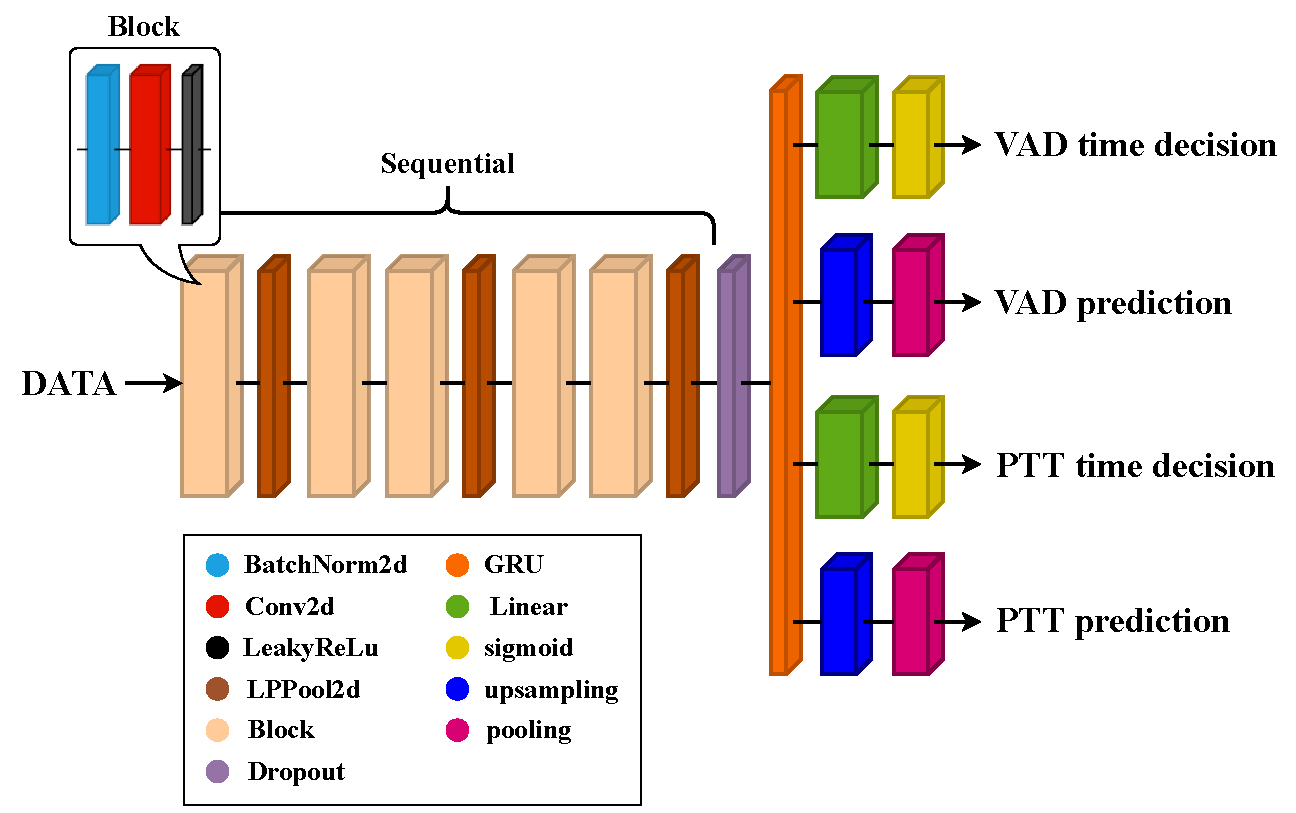
\includegraphics[width = \textwidth]{obrazky-figures/GPVAD_arch.pdf}
        \caption{Adapted CRNN model from GPVAD implementation. The time decision represents a~frame-level prediction for the frame being a~certain class. The overall prediction outputs represent the probability of each event happening in the audio. }
        \label{fig:gpvadarch}
    \end{figure}
    
    CRNN architecture has many two-dimensional convolutional layers as well as pooling layers and a~recursive unit. Convolutional layers in combination with the recursive unit have proven themselves useful in supervised training for voice activity detection. The architecture is the same as before the adaptation, but now it contains one additional output layer for PTT detection. The adaptation of this model consisted of adding another layer to the output layer, which served the purpose of PTT detection. 
    
    Input to this model is a~Mel spectrogram as well, but with different parameters, as shown in section \ref{Dataset NN}. 
    The output of this neural network is a~time decision for each frame of the audio for voice activity and push-to-talk events. Time decision for voice activity represents a~two-dimensional array that contains the probability of each speech and non-speech event determined individually for each class. The neural network provides time decisions for PTT as well. The clip output represents the overall probability of each event occurring in the audio.

    The process of extracting features remained unchanged. On the other hand, the process of creating labels was slightly modified. Voice activity labels are generated from predictions of a~pre-trained neural network. PTT frame labels are created by using the PEEK algorithm, which was explained in subsection \ref{LabelPTT}. These frames labels are nearly 100\% accurate (see \ref{tab:comparisionapproaches}).
    The clip level was created by using a~linear pooling function on frame-level labels. 

    The training process, which will be further explained in chapter \ref{Experiments} needed adjustments too. The data loading process was modified to load these new labels. 
    The loss function which was computed on the frame level was modified to compute loss for each VAD and PTT output correspondingly. 

    GPVAD approach contained lots of implementation mistakes. These mistakes did not influence the overall performance of the model, but because of them, the adaptation was quite complicated. The main problems were incorrectly named files and missing files in some directories. Repairing the implementation needed knowledge of the whole project. The overall performance is sufficient, but according to the manual some things did not work, and it was necessary to re-implement them. Problems and resolutions will be further discussed in chapter \ref{Experiments}.

    \vspace{0.2cm}


    This chapter provided an overview of the used models in the thesis. Two architectures of neural networks were introduced. The models are suited for voice activity and push-to-talk detection. The models were proposed in order to get familiar with machine learning. 

    Finally, an introduction to GPVAD was provided. GPVAD is a~neural network which is capable of detecting speech even in a~noisy environment. This model is adapted to match proposed experiments. 


    
%=========================================================================

\chapter{Experiments and Evaluations}\label{Experiments}

    This chapter provides a~complete overview of all experiments. The training process of the neural networks will be described, and the distribution of the dataset as well. It will discuss used evaluation metrics. Finally, a~comparison between models will be provided. 

\section{Evaluation Metrics}\label{Eval Metrics}

    Evaluation metrics are utilised in two stages in a~basic classification problem: training and testing. 
    
    Metrics are used to enhance the classification algorithm during the training stage. They can be used as discriminators to determine and select optimal solutions that can predict future evaluations more accurately.  
    Metrics are used in the testing phase to evaluate the overall performance and effectiveness of the classifier on unseen data. 
    
    Each stage requires a~dataset containing previously unseen data. Unseen data are commonly divided into test and validation datasets. After training, a~test dataset is used to evaluate the model's performance. 

    Computing a~loss function and accuracy on a~validation dataset are common techniques for evaluating the progress of neural network learning. The validation dataset contains data that was not included in the training set in order to test whether the model is improving in its predictions for previously unknown data. If the validation loss value starts increasing, it indicates that the model is starting to overfit the training data and that training should be interrupted.

    Following the training process, the model is evaluated on the test dataset. It is determined by how well the model predicts and how general it is. 

    Some of the most common evaluation metrics \cite{FAWCETT2006861} used for confirming whether a~model proves to be accurate are:
    \begin{itemize}
        \item \textbf{Accuracy} computation is the most commonly used method for determining model correctness. It is a~ratio of the correct predictions or named as True Positive (TP) and True Negative (TN) over all evaluated instances, meaning over False Positive (FP) and False Negative (FN) predictions as well \ref{acceq}. 
        \begin{equation}\label{acceq}
            \frac{TP+TN}{TP+FP+TN+FN}
        \end{equation}
         \newpage
        \item \textbf{Precision} (P) value is representing a~ratio between actual or True Positive (TP) values and all predicted positive values from the model, including False Positive (FP) predictions \ref{precisioneq}. 
        \begin{equation}\label{precisioneq}
            \mathrm{P}=\frac{\mathrm{TP}}{\mathrm{TP}+\mathrm{FP}}
        \end{equation}
        \item \textbf{Recall} (R) is a~value obtained by calculating how many True Positives (TP) were predicted by the model. False Negative (FP) values represent incorrect negative predictions \ref{recalleq}.
        \begin{equation}\label{recalleq}
            \mathrm{R}=\frac{\mathrm{TP}}{\mathrm{TP}+\mathrm{FN}}
        \end{equation}
        \item \textbf{F1 score} represents a~mean value of precision and recall \ref{F1scoreeq}. 
        \begin{equation}\label{F1scoreeq}
            F 1=2 \cdot \frac{\mathrm{PR}}{\mathrm{P}+\mathrm{R}}
        \end{equation}
        \item \textbf{Confusion matrix} represents a~summary of each True Positive (TP), False Positive (FP), False Negative (FN) and True Negative (TN) prediction on currently evaluated data (table \ref{confusionmatrix}). 
        \begin{table}[!h]
        \begin{center}
        \begin{tabular}{|c|c|c|}\hline 
            & \textbf{True Positive Class} & \textbf{True Negative Class} \\ \hline
            \textbf{Predicted Positive Class} & TP & FP \\ \hline
            \textbf{Predicted Negative Class} & FN & TN \\ \hline
        \end{tabular}
        \caption{Confusion matrix structure.}
        \label{confusionmatrix}
        \end{center}
        \end{table}
        \item \textbf{AUC-ROC} method reflects the overall performance of a~classifier. AUC or the area under a~ROC\footnote{Receiver operating characteristic.} curve is a~value in a~range [0.5,1.0] where 0.5 corresponds to a~random classifier and 1.0 to a~perfect classifier. The ROC curve is the trade-off between True Positives (TPR) and False Positives (FPR) (figure \ref{fig:AUCROCexample}).

        \begin{figure}[ht!]
            \centering
            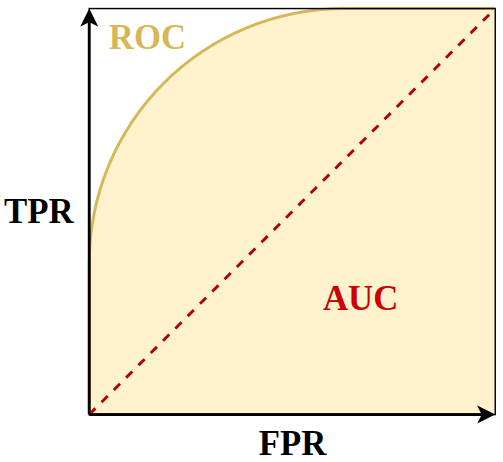
\includegraphics[width = 0.45\textwidth]{obrazky-figures/AUC-ROC.png}
            \caption{AUC-ROC curve.}
            \label{fig:AUCROCexample}
        \end{figure}
    \end{itemize}

\newpage

\section{Training and Validation of Selected Models}

    The training process of the neural network can be really challenging task. Various factors affect the training process. A~careful selection of hyperparameters needs to be done. Dataset robustness is also a~huge factor to determine whether the training was successful or not. Generally speaking the more data the better performance of the model. High-quality labels are crucial in supervised training. 

    The process of training the neural networks in this thesis consisted of data pre-processing, which includes feature extraction and label generation.

    This section is divided into two parts. The first part (see \ref{TVEM}) will talk about the training and validation process of proposed experimental models. These models will then be evaluated and compared with each other. The second part (see \ref{TVGM})  will talk about the training process of GPVAD reimplementation. It will include an overview of the model's performance without adding another layer for push-to-talk detection. Later, the fine-tuning process will be explained. 
    
    Finally, the accuracy of these models will be compared in section \ref{final comparison}

    All the training process was done on GPU. The dataset was divided into three parts. Training data represented 70\% of the dataset, and the testing and validation set both represented 15\%. 

    In the unaltered ATCO2 dataset, the class distribution is 65\% for speech and 35\% for non-speech. This is not necessarily the best balance of the two classes, so it needed to be altered.
    The specific numbers can be found in the following table:

    \vspace{0.2cm}

    \begin{table}[!h]
        \begin{center}
        \begin{tabular}{|c|c|c|}\hline 
            & \textbf{Speech (\%)} & \textbf{Non-Speech (\%)} \\ \hline
            \textbf{Training Data} & 47.60 & 22.40 \\ \hline
            \textbf{Testing Data} & 10.20 & 4.80 \\ \hline
            \textbf{Validation Data} & 10.20 & 4.80 \\ \hline
        \end{tabular}
        \caption{Speech and non-speech frames distribution in the original ATCO2 dataset without changes.}
        \label{tableVAD}
        \end{center}
    \end{table}
    
    In the ATCO2 dataset, PTT frames have significantly lower representation than other classes (table \ref{tableATCO2distrib}).

    \begin{table}[!h]
        \begin{center}
        \begin{tabular}{|c|c|c|c|}\hline 
            & \textbf{Speech (\%)} & \textbf{Non-Speech (\%)} & \textbf{Push-To-Talk (\%)} \\ \hline
            \textbf{ATCO2 Dataset} & 66.35 & 32.81 & 0.83 \\ \hline
        \end{tabular}
        \caption{Speech, non-speech and push-to-talk frames distribution in the original ATCO2 dataset without changes.}
        \label{tableATCO2distrib}
        \end{center}
    \end{table}

    \newpage

    \subsection{Training and Validation of Experimental Models}\label{TVEM}

    It is necessary to define some concepts first. FNN is an abbreviation for feed-forward neural network, which was proposed in section \ref{ENNarch}. CNN is a~neural network that processes input frames as a~two-dimensional array (see \ref{fig:CNN2D}). The models require a~proper dataset, on which they can be learnt.

    After the neural network's architecture has been established and the data has been pre-processed and labelled, the training phase can officially start. It is vital to note that this procedure takes quite a~while because an ideal solution is rarely found on the first try. Experimenting and analysing neural networks is time-consuming. 
    
    \subsubsection{Feed-Forward Neural Network}\label{FNNtrainandvalid}

    The simple feed-forward model is trained first. There are three experiments in total:
    \begin{itemize}
        \item \textbf{Experiment A}: only on Voice activity detection (see \ref{expA}).
        \item \textbf{Experiment B}: only on Push-to-talk detection (see \ref{expB}).
        \item \textbf{Experiment C}: on both Push-to-talk and voice activity detection (see \ref{expC}).
    \end{itemize}

    Selected hyperparameters are shown in the following table:
    
    \begin{table}[!h]
    \begin{center}
    \begin{tabular}{|c|c|c|c|c|c|}\hline 
        & \textbf{LR} & \textbf{LF} & \textbf{Optimizer} & \textbf{BS} & \textbf{Epochs} \\ \hline
        \textbf{FNN} & 0.001 & Cross Entropy & Adam & 32 & 5 \\ \hline
    \end{tabular}
    \caption{Hyperparameters for FNN training. LR – learning rate, LF – loss function, BS – Batch Size.}
    \label{tableparameters}
    \end{center}
    \end{table}

    To use regularization of the training as well, an \textit{Early Stop} mechanism was added to the process. The Early Stop is initialised with a~minimal difference of 0.15 and patience 10. This method focuses on terminating training before overfitting. Overfitting is a~frequent problem in the training of neural networks. This happens when the model has learned to predict the training data perfectly but is unable to predict the new, unknown data. This indicates that the model failed to generalise the data. 
    
    To experiment with neural networks, the model was first trained solely to predict speech activity. 

    Experiment A, which concentrated on VAD was trained on approximately 90,000 frames with distribution between speech and non-speech was 50\% for each class. For experiment B, the number of frames was reduced to approximately 40,000 with 50\% for push-to-talk and 50\% for non-push-to-talk. Finally, for experiment C, the number of data frames is approximately 50,000. 

    Each evaluation is done by comparing frame to frame. This leads to a~more precise evaluation on a~frame level.

    \newpage
    \subsubsection{Experiment A}\label{expA}

    For experiment A, the dataset was limited to around 90,000 frames with a~distribution of 50\% for each class. The frames were divided into training, testing and validation data by recordings to avoid providing the neural network by mistake in neighbouring frames. The distributed frames were shuffled.

    The accuracy of this neural network after one epoch is 77.2\% which is pretty sufficient for the first try. Precision and Recall of this neural network is around 80\% for each.  
    
    Despite the fact that the architecture was simple, and the dataset was relatively small, the results were satisfactory. Speech is labelled with value one and non-speech with value zero. The training was done in one epoch.

    Validation of the neural network on an unknown recording resulted in 88.9\% accuracy. This accuracy was calculated by comparing the labels from \texttt{CNET} file and an index of softmax output from the neural network with higher (figure \ref{fig:validationFNN}).

    \begin{figure}[ht!]
        \centering
        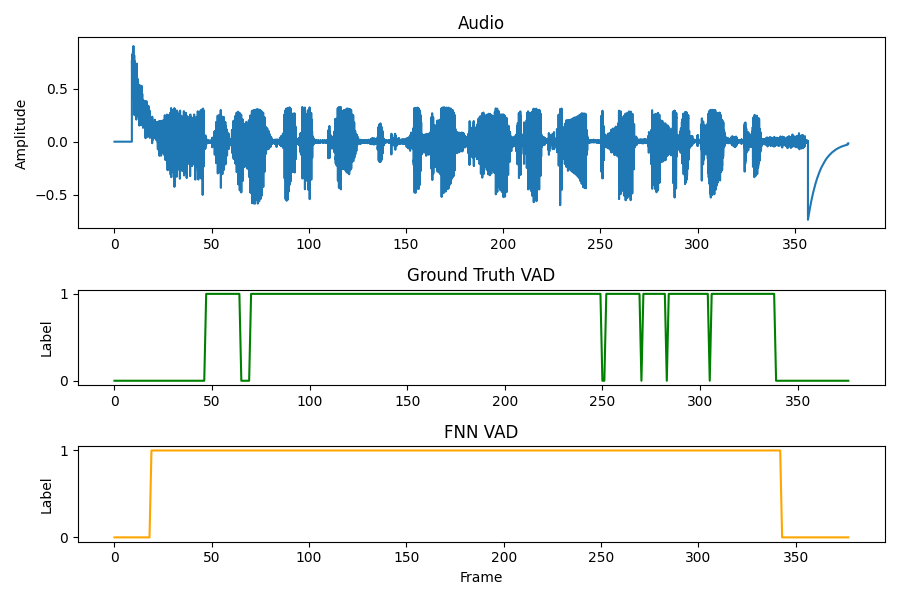
\includegraphics[width = \textwidth]{obrazky-figures/FNNOUTPUT_10.png}
        \caption{Experiment A: Validation of unknown audio on voice activity detection.}
        \label{fig:validationFNN}
    \end{figure}
    \newpage
    \subsubsection{Experiment B}\label{expB}

    Experiment B dwells in training the FNN only on push-to-talk detection, without distinguishing speech and non-speech frames. The distribution between push-to-talk and non-push-to-talk classes is 50\% for each. Non-push-to-talk frames were randomly selected from a~set of speech and non-speech frames to match the length of the PTT set. This may not be the perfect distribution considering that the validation data will never contain a~recording in which 50\% is a~push-to-talk event, but for this experiment, it was not taken into consideration. Modification of the distribution will be taken into consideration in section \ref{TVGM}. The hyperparameters for training remained the same as were in the first experiment. The accuracy of this neural network on the test dataset is 96.6\%.

    Validating neural network on unknown recording resulted in 99.3\% (figure \ref{fig:validationFNN12}). Despite a~few false alarms, the overall performance is decent.

    \begin{figure}[ht!]
        \centering
        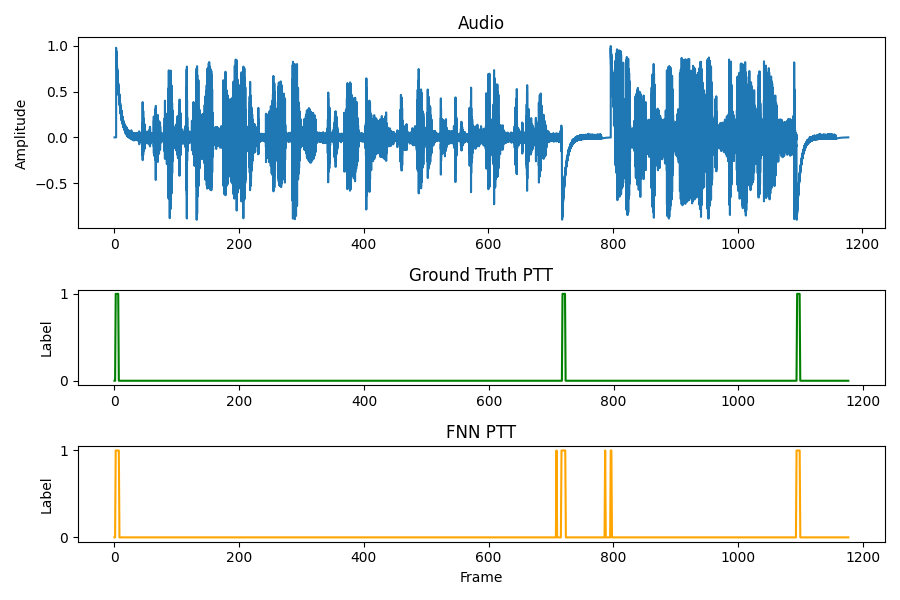
\includegraphics[width = \textwidth]{obrazky-figures/FNNOUTPUT_12.png}
        \caption{Experiment B: Validation of unknown audio on push-to-talk detection.}
        \label{fig:validationFNN12}
    \end{figure}

    \newpage
    
    \subsubsection{Experiment C}\label{expC}
    
    For experiment C, another output layer was added to the neural network to detect both push-to-talk and voice activity at the same time. 

    Every PTT frame was stored, and speech and non-speech frames were chosen randomly to match the length of the PTT frames. Because the final evaluation is done on audio recordings which contain more non-push-to-talk frames, the distribution of the classes was altered. The ratio between speech and non-speech frames remained the same. Push-to-talk frames represented 20\% of the dataset. 
    
    This distribution is probably not the most balanced, but for now, it is sufficient.
    Training the neural network resulted in a~94.10\% accuracy for push-to-talk detection and 64.88\% for voice activity detection. The early stop regularisation element was triggered during the third epoch. Validating the whole audio with PTT events ended up as a~partial success because of one false alarm for push-to-talk (figure~\ref{fig:validationFNNMLT}). FNN with 99.15\% accuracy predicted locations of push-to-talk events and with 74.26\% accuracy predicted speech segments on unknown audio. This accuracy is discussable due to marking nearly everything in the signal as a~speech. 
    
    \begin{figure}[ht!]
        \centering
        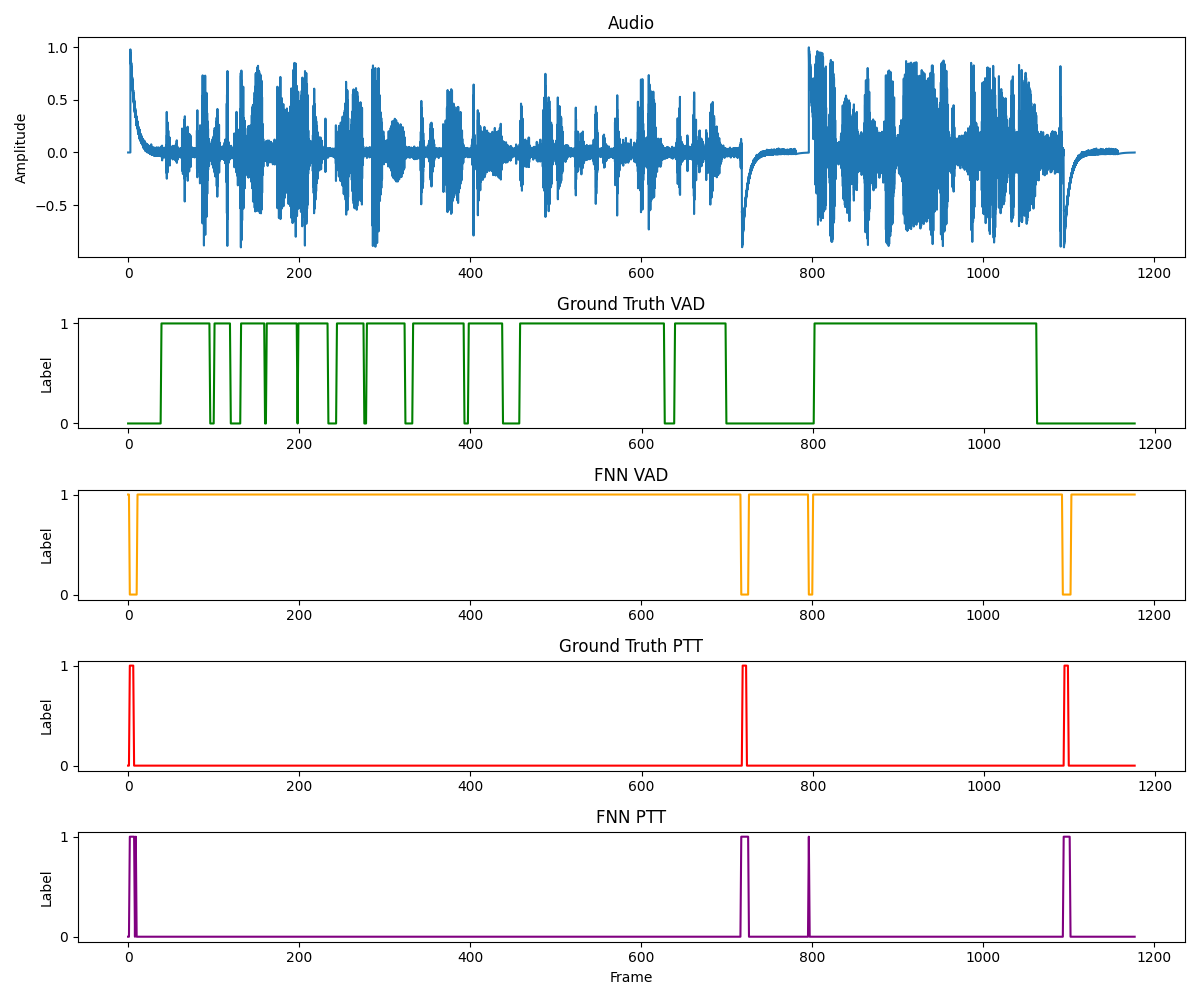
\includegraphics[width = \textwidth]{obrazky-figures/FNNOUTPUT_MTL.png}
        \caption{Experiment C: Validation of unknown audio on voice activity and push-to-talk detection.}
        \label{fig:validationFNNMLT}
    \end{figure}

    \newpage
    For this experiment, the ROC curve was calculated on each task \ref{fig:validationFNNMLTROC}. A~Receiver Operating Characteristic Curve (ROC) is a~common method for summarising classifier performance across a~range of true positive (TP) and false positive (FP) error rates \cite{swets1988}.
    
        
    \begin{figure}[ht!]
        \centering
        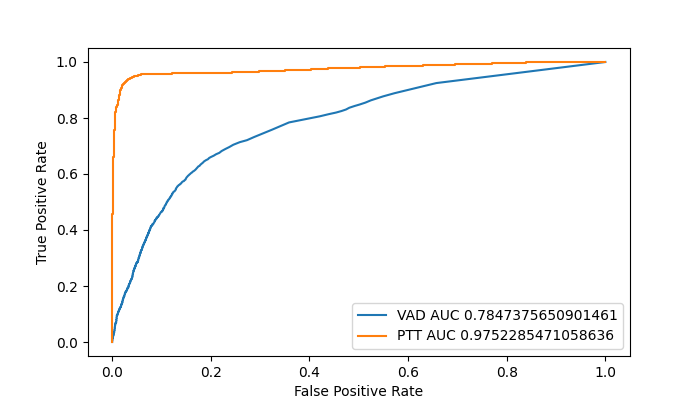
\includegraphics[width = \textwidth]{obrazky-figures/ROC.png}
        \caption{AUC-ROC evaluation.}
        \label{fig:validationFNNMLTROC}
    \end{figure}

    
    In summary, FNN performed with \textbf{77.21\%} on voice activity detection (Experiment A), \textbf{96.60\%} on push-to-talk (Experiment B) and \textbf{94.10\%} for push-to-talk and \textbf{64.88\%} on multitasking (Experiment C).
    
    The models were trained approximately for one hour and used almost 1 GiB of memory on the GPU. 
    
    Because this feed-forward architecture served only as a~stepping stone, it was unnecessary to continue with experiments on this architecture. 

    \newpage

    \subsubsection{Convolutional Neural Network}

    The second experimental neural network is a~convolutional neural network fed by signal frames kept in a~two-dimensional array. This neural network could possess an advantage over the FNN thanks to its convolutional layers.

    This CNN model is trained only on multitasking for two epochs. The training process was done on  the same dataset, as it was used for experiment C (see \ref{expC}).

    The hyperparameters are presented in the following table:

    \begin{table}[!h]
    \begin{center}
    \begin{tabular}{|c|c|c|c|c|c|}\hline 
        & \textbf{LR} & \textbf{LF} & \textbf{Optimizer} & \textbf{BS} & \textbf{Epochs} \\ \hline
        \textbf{FNN} & 0.001 & Cross Entropy & Adam & 32 & 5\\ \hline
    \end{tabular}
    \caption{Hyperparameters for CNN training. LR – learning rate, LF – loss function, BS – Batch Size.}
    \label{tableparametersCNN}
    \end{center}
    \end{table}
    
    
    After testing the neural network on a~test dataset, the accuracy of the CNN model is 96.80\% for push-to-talk detection and 82.00\% for voice activity detection. Validating the model on the unknown audio resulted in 99.40\% accuracy for push-to-talk and 87.59\% for voice activity (figure \ref{fig:validationCNNMLT}).

    \begin{figure}[ht!]
        \centering
        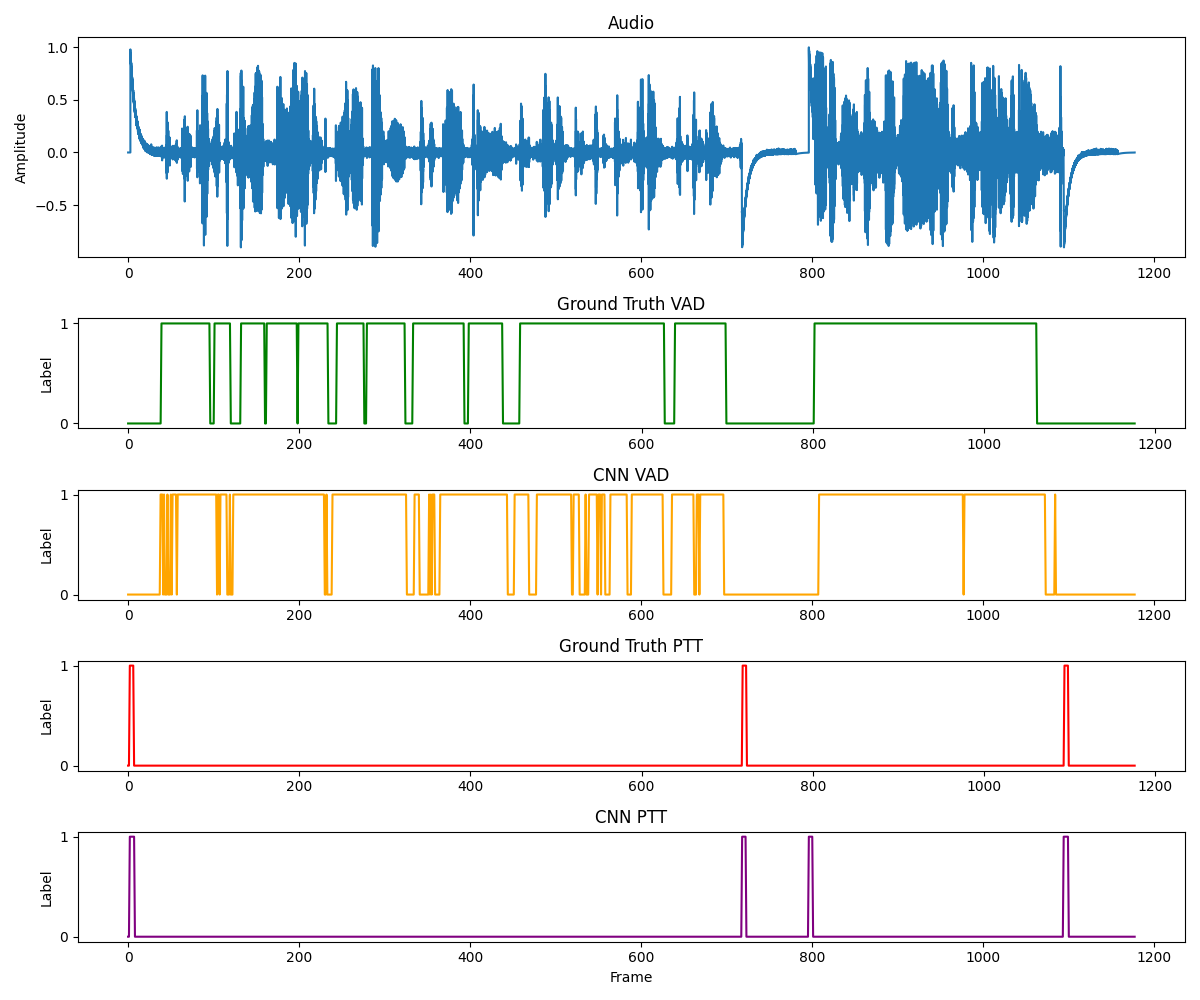
\includegraphics[width = \textwidth]{obrazky-figures/CNNOUTPUT_MTL.png}
        \caption{Validation of unknown audio on voice activity and push-to-talk detection.}
        \label{fig:validationCNNMLT}
    \end{figure}

    The AUC-ROC evaluation resulted in 0.89 for voice activity detection and 0.978 for push-to-talk (figure \ref{fig:ROCMLTCNN}). The evaluation was computed by a~function from \texttt{sklearn} library\footnote{see
    \href{scikit-learn.org/stable/modules/generated/sklearn.metrics.auc.html}{\texttt{scikit-learn.org/stable/modules/generated/sklearn.metrics.auc.html}}}.
    
    \begin{figure}[ht!]
        \centering
        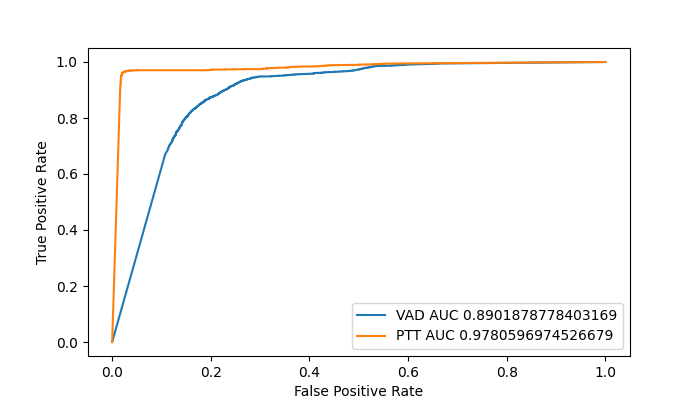
\includegraphics[width = \textwidth]{obrazky-figures/ROCCNN.png}
        \caption{AUC-ROC evaluation curve computed on both push-to-talk and voice activity detection.}
        \label{fig:ROCMLTCNN}
    \end{figure}

    a~confusion matrix was employed to evaluate the correctness of the model (figure \ref{fig:confusionmatrixcnn}). The matrix's values represent average values over every batch in the test dataset. 
 
    \begin{figure}[ht!]
        \centering
        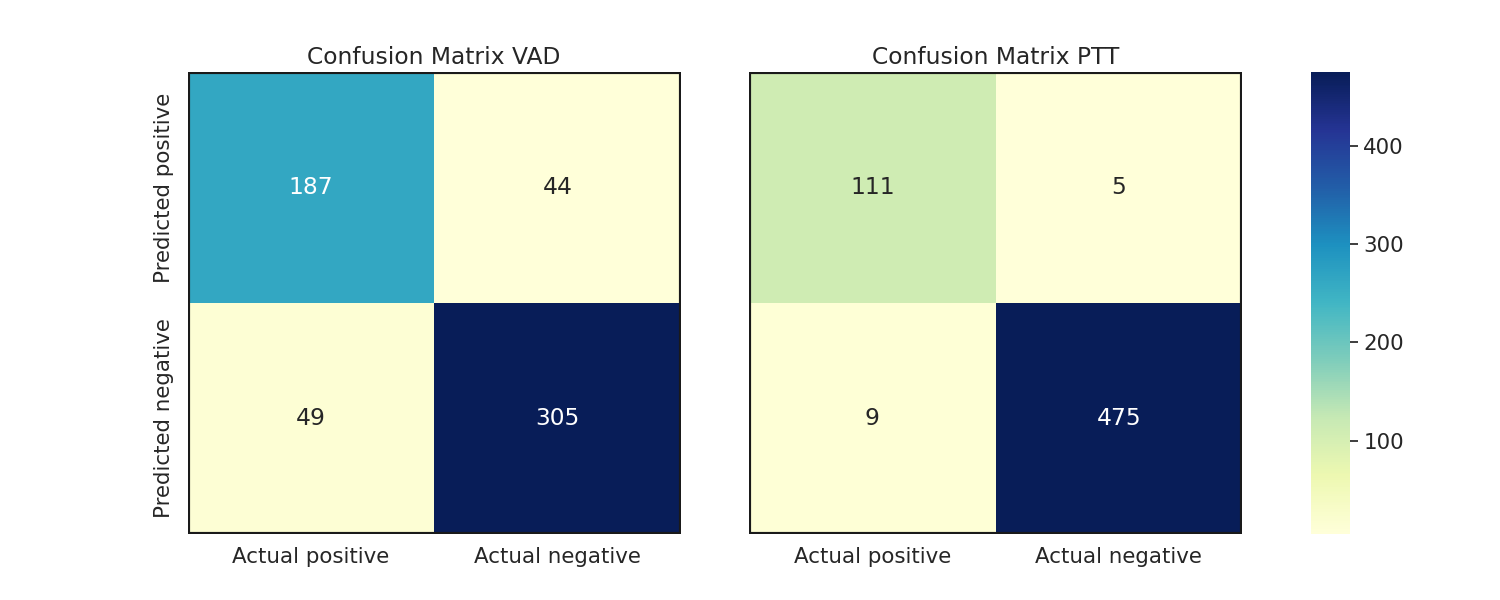
\includegraphics[width = \textwidth]{obrazky-figures/CM_VAD_PTT.png}
        \caption{Confusion matrix of the model for each task.}
        \label{fig:confusionmatrixcnn}
    \end{figure}
    The model was trained for approximately  half an hour with a~memory usage of 900 MiB on GPU. 
    \newpage

    After training the proposed experimental models, a~comparison between each result is needed. Firstly, the three experiments on the FNN model are evaluated.

    \begin{table}[!h]  
    \begin{center}
    \begin{tabular}{|c|c|c|c|c|c|c|}\hline 
        \multicolumn{2}{|c|}{} & \textbf{Acc. (\%)}  & \textbf{Rec. (\%)} & \textbf{Prec. (\%)} & \textbf{F1 (\%)} & \textbf{AUC}\\ \hline
        \textbf{A} & \textbf{VAD} & 77.21 & 79.00 & 85.70 & 82.20 & 0.718\\ \hline
        \textbf{B} & \textbf{PTT} & 96.60 & 91.30 & 92.50 & 91.30 & 0.977\\ \hline
        \multirow{2}{*}{\textbf{C}} & \textbf{VAD} & 64.88 & 39.40 & 72.50 & 50.90 & 0.780\\ \cline{2-7}
        & \textbf{PTT} & 94.10 & 91.86 & 86.00 & 87.80 & 0.975\\ \hline
    \end{tabular}
    \caption{Evaluation metrics of FNN model on different experiments.}
    \label{evaluationFNN}
    \end{center}
    \end{table}

    Table \ref{evaluationFNN} represents evaluation metrics for each experiment mentioned earlier in this section. Each percentage is an average value over test batches results. They could not be compared due to being learned for different tasks, but the overall most successful experiment with this architecture was the experiment with push-to-talk detection. 
    

    FNN and CNN were trained to provide multitask predictions under the same conditions and with the same dataset.
    It is possible to compare their performance (table \ref{comparisonFNNCNN}). All of the values are an average of each metric over every test batch. 

    \begin{table}[!h]  
    \begin{center}
    \begin{tabular}{|c|c|c|c|c|c|c|}\hline 
        \multicolumn{2}{|c|}{} & \textbf{Acc. (\%)}  & \textbf{Rec. (\%)} & \textbf{Prec. (\%)} & \textbf{F1 (\%)} & \textbf{AUC} \\ \hline
        \multirow{2}{*}{\textbf{FNN}} & \textbf{PTT} & 94.10 & 91.86 & 86.00 & 87.80 & 0.975\\ \cline{2-7}
        & \textbf{VAD} & 64.88 & 39.40 & 72.50 & 50.90 & 0.780\\ \hline
        \multirow{2}{*}{\textbf{CNN}} & \textbf{PTT} & 96.88 & 94.24 & 90.33 & 92.06 & 0.978\\ \cline{2-7}
        & \textbf{VAD} & 81.99 & 81.12 & 77.98 & 79.47 & 0.890\\ \hline
    \end{tabular}
    \caption{Evaluation metrics of FNN and CNN models. The comparison on task is provided individually.}
    \label{comparisonFNNCNN}
    \end{center}
    \end{table}

    It is possible to state, that architecture with convolutional layers helped the model to predict more correct outputs. The most noticeable difference between the FNN approach and the CNN approach is validation on audio, which does not contain any PTT event. The CNN model can accurately mark each frame as not push-to-talk, but FNN causes one or two false alarms. 


    \newpage
    
    \subsection{Training and Validation of GPVAD Model}\label{TVGM}

    The GPVAD implementation provides an effective pre-trained model for voice activity detection. This model was trained on a~large amount of data and can correctly distinguish speech segments. The GPVAD CRNN architecture is complex and contains various layers such as convolutional layers and a~recurrent unit. 


    The main difference between GPVAD's training and training on experimental models is that the input to the models does not consist of a~group of local frames, but rather a~global group of frames in the whole audio (see chapter \ref{Data}). This provides a~context for the neural network on a~global level of the whole audio. 


    An architecture of the CRNN model was used in order to train the neural network on push-to-talk detection. A~dataset for this training consisted of various audio recordings. These recordings are divided into two classes, one that contains no push-to-talk event and a~second that contains at least one. The ratio between frames that contain push-to-talk events and ones that do not contain the event is 10:90. This seemed reasonable because the final evaluation or usage of this model is for audio recordings that do not contain a~big amount of push-to-talk events. When training on balanced distribution, the results were poor. Experimenting with various distributions resulted in choosing approximately a~10:90 ratio. 
    
    The overall number of recordings for this training was 1000. Each recording was approximately 2 seconds long. The whole dataset is something little over 30 minutes long.

    \begin{table}[!h]
    \begin{center}
    \begin{tabular}{|c|c|c|c|c|}\hline 
        \multirow{2}{*}{} & \multicolumn{2}{c|}{\textbf{Push-To-Talk}} & \multicolumn{2}{c|}{\textbf{Non-PTT}}\\\cline{2-5}
         & \textbf{Frames (\%)} & \textbf{Recording (\%)} & \textbf{Frames (\%)} & \textbf{Recordings (\%)} \\ \hline
         \textbf{Dataset} & 11.55 & 58.60 & 88.45 & 41.40 \\ \hline
    \end{tabular}
    \caption{Dataset distribution.}
    \label{tableparametersGPVAD}
    \end{center}
    \end{table}

    The push-to-talk event lasts for 100 ms. During label generation, it is also checked if the peak in the frame is not too close to the end of the frame. This could possibly trigger a~false alarm because a~majority of the frame is the non-push-to-talk segment. If the peak\footnote{Peak is a~specific sample that was considered as local maximum by the PEEK algorithm provided in the chapter \ref{Data}.} is in the last 15\% of the frame, the frame is considered non-push-to-talk. 


    The hyperparameters for this training are shown in the table \ref{tableparametersGPVAD}. The training was done in 10 epochs.
    
    \begin{table}[!h]
    \begin{center}
    \begin{tabular}{|c|c|c|c|c|}\hline 
        & \textbf{Learning Rate} & \textbf{Loss Function} & \textbf{Optimizer} & \textbf{Batch-Size} \\ \hline
        \textbf{GPVAD PTT} & 0.001 & Cross Entropy & Adam & 64 \\ \hline
    \end{tabular}
    \caption{Hyperparameters for GPVAD training.}
    \label{tableparametersGPVAD}
    \end{center}
    \end{table}

    \newpage
   
    Weights were initialised by loading one of the provided models in the GPVAD implementations.  
    The training process of this model resulted in 83\% accuracy and 80\% F1 score. 
    The model was validated on audio and resulted in 94.7\% accuracy \ref{fig:validationgpvadptt}. 

    \begin{figure}[ht!]
        \centering
        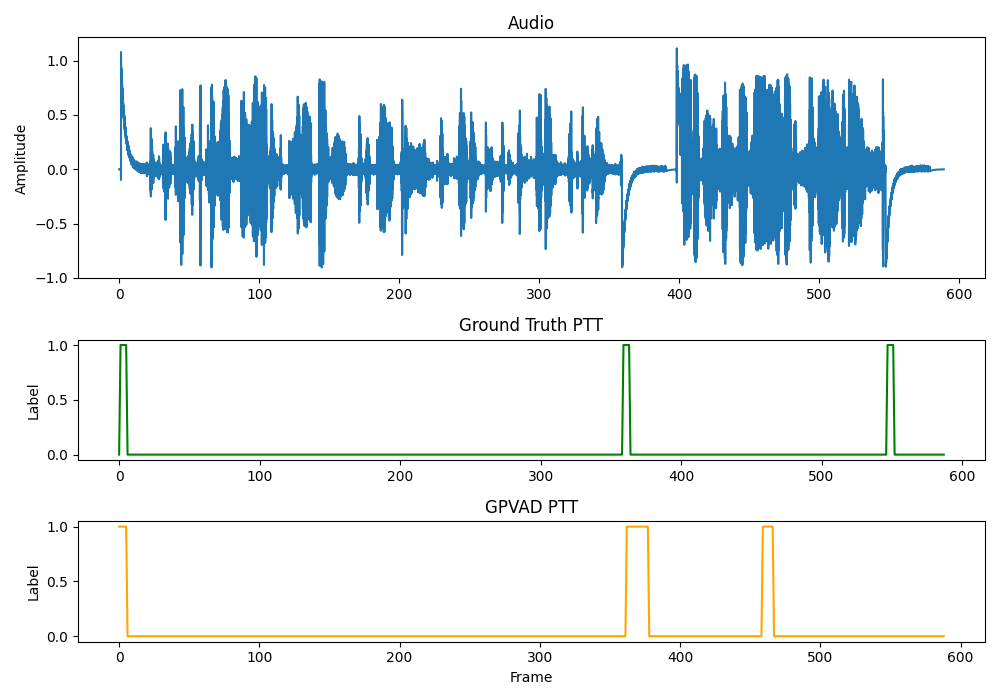
\includegraphics[width = \textwidth]{obrazky-figures/GPVADPTT.png}
        \caption{Validation of unknown audio on push-to-talk detection.}
        \label{fig:validationgpvadptt}
    \end{figure}


    Finally, a~GPVAD with adaptation to predict clip level and frame level predictions for push-to-talk is trained. The hyperparameters remain the same as for push-to-talk training (table \ref{tableparametersGPVAD}) except for the learning rate. The learning rate changed to 0.01. The dataset distribution needed to be changed to be more balanced. The previously mentioned ratio was not suitable for this training and the training resulted in many false negative predictions due to lack of PTT events. The dataset was augmented, so it doubled in the number of recordings. The dataset contained 6000 audio files which represent nearly three and a~half hours. The distribution on the first dataset was not sufficient for this problem. 

    The weights were initialised by loading the \texttt{sre} model provided in the GPVAD implementation. This model can accurately predict speech segments, detect speech in noisy environments and can localise speech that is very quiet. The model is a~good starting point in order to train a~multitask model. 

    The training process lasted 50 epochs and resulted in a~maximum of 66\% accuracy in detecting the push-to-talk signal on a~dataset with a~35:65\footnote{push-to-talk frames : non-push-to-talk frames} ratio. The fine-tuning model only on the last output layer was challenging. The neural network was inclined in predicting more non-push-to-talk events than the ground truth. When providing a~dataset with a~larger representation of push-to-talk events, the model was still inclined to predict non-push-to-talk events. 
    
    \newpage
    Even though the weights of the new output layer look ``healthy'' with majority begin low weights (figure \ref{fig:weightsoutput1}) \cite{applyingnn}. The distribution of weights mimics the Gaussian distribution.  
    
    \begin{figure}[ht!]
        \centering
        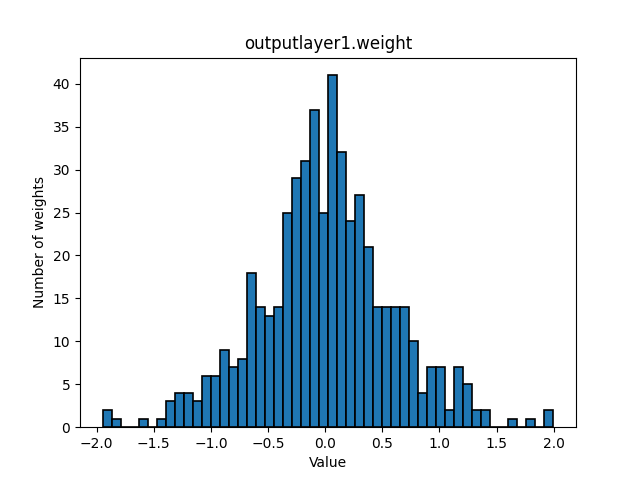
\includegraphics[width = 0.7\textwidth]{obrazky-figures/histogramoutputlayer1.png}
        \caption{Histogram of weights on the new output layer for push-to-talk detection.}
        \label{fig:weightsoutput1}
    \end{figure}

    For post-processing, the only threshold that was used was if the PTT prediction is higher than the non-PTT prediction. This resulted in 93.9\% accuracy but caused a~false alarm during a~speech segment and missed one push-to-talk, so it is discussable to take it into consideration (figure \ref{fig:gpvadoutputmlt}). 

    \begin{figure}[ht!]
        \centering
        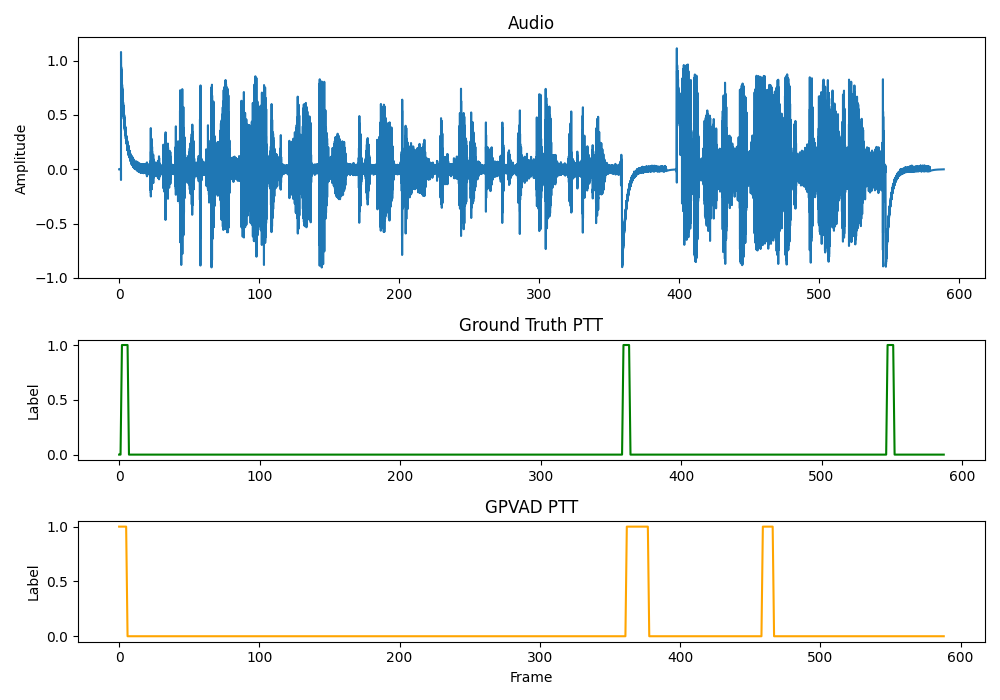
\includegraphics[width = 0.85\textwidth]{obrazky-figures/GPVADMLT.png}
        \caption{Validation of unknown audio on voice activity and push-to-talk detection.}
        \label{fig:gpvadoutputmlt}
    \end{figure}


\newpage

\section{Comparison Between Different Approaches}\label{final comparison}


    In this section, the used models are compared. The comparison can't be done the exact way as the FNN Experiment C and CNN because GPVAD was pre-trained with much more data. The baseline evaluation metrics for the used model \texttt{sre} are provided in the following table: 

    \begin{table}[!h]
    \begin{center}
    \begin{tabular}{|c|c|c|c|c|c|}\hline 
        & \textbf{Prec. (\%)} & \textbf{Rec. (\%)} & \textbf{F1 (\%)} & \textbf{AUC} \\ \hline
        \textbf{aurora\_clean}  & 96.844 & 95.102 & 95.93  & 98.66\\ \hline
        \textbf{aurora\_noisy}  & 90.435 & 92.871 &	91.544 & 97.63\\ \hline
        \textbf{dcase18}        & 89.202 & 88.362 &	88.717 & 95.2  \\ \hline 
    \end{tabular}
    \caption{The evaluation metrics for baseline model on different datasets, which is further explained in the original GPVAD paper.}
    \label{baselinegpvad}
    \end{center}
    \end{table}

    CNN, FNN and GPVAD required different datasets in order to learn given tasks. The CNN and FNN were trained from scratch so they needed a~reasonable distribution between all four classes. On the other hand, the GPVAD was fine-tuned on push-to-talk detection, so the dataset needed to be more robust on push-to-talk events. 

    Despite that at least some comparison can be provided. The FNN model achieved 94.10\% accuracy for PTT detection and 64.88\% for voice activity detection. The CNN model resulted in \textbf{96.88\%} accuracy for push-to-talk detection and \textbf{81.99\%} for voice activity detection. The GPVAD achieved 66\% accuracy for push-to-talk detection. 

    This makes the CNN model the best in terms of performance and size. The model consists of 224,032 learnable parameters. GPVAD contains 677,569 learnable parameters. 

    The best model for sole push-to-talk detection is GPVAD with \textbf{83\%} accuracy. 

    The honourable mention does to the proposed PEEK algorithm, which was crucial to achieving these results. 
 
    
\section{Possible Improvements and Future Work}\label{improvements}

    GPVAD adaptation provided sufficient results. The next step in fine-tuning the model can involve experimenting with freezing only some weights. Another possible improvement is to experiment further with proper data distribution to obtain the most optimal and correct results.
    Due to inclining to the non-push-to-talk event, a~weighted training could be efficient. 

    To enhance CNN correctness, a~bigger and more robust dataset could be provided to achieve even better results. 

    After adjusting these two models, the proposed solution could help with detecting voice activity and push-to-talk segments in air traffic communication. 
    
    Another possible approach to detect push-to-talk events is to train a~neural network with an unsupervised method and provide data which contain silence or push-to-talk event. 

%=========================================================================

\chapter{Conclusion}\label{Conclusion}

    The main goal of this thesis was to implement and evaluate models that are suitable for voice activity and push-to-talk detection. 
    To properly train the neural network, it is necessary to provide an accurate and robust dataset. The ATCO2 dataset contained four hours of air traffic communication and was suitable for this task. The recordings consisted of 65\% speech segments and 35\% non-speech segments. 
    
    Converting audio files into Mel spectrograms is a~common approach for training neural networks. Supervised training requires proper and correct labels. All the labels were frame-level. For experimental models, voice activity detection labels were extracted from files in the ATCO2 dataset archive. The labels for GPVAD training were obtained by prediction from their \textit{sre} model. Push-to-talk events were not labelled, so an algorithm needed to be invented. The best approach lies in localising the local extrema and then selecting only those from which the signal has at least 100 ms of negative amplitude and is the only peak in the closest frame.
    
    Processed data was used to train the neural networks. The two experimental architectures were a~basic feed-forward neural network and a~simple convolutional neural network. To get familiar with neural networks, the feed-forward model was the stepping stone, and various experiments were tried. This model was trained on push-to-talk and voice activity detection separately as well as in combination. The accuracies of this model were 77.2\% for voice activity detection, 96.6\% for push-to-talk detection and 83\% for both push-to-talk and voice activity detection. The CNN model was trained only for multitask predictions and resulted in 90\% accuracy. 
    
    The final solution was created through the adaptation of the GPVAD implementation. The GPVAD approach has accurate results for voice activity detection and was a~suitable choice for this task. 
    
    The architecture of GPVAD was used for training on push-to-talk detection separately. With loading the \textit{sre} model as starting point, the accuracy of this model is 83\% and can provide sufficient predictions for push-to-talk events. The final multitasking neural network was trained and the model \textit{sre} was used as starting point as well. An additional output layer was added for clip and frame level prediction. This resulted in 66\% accuracy for push-to-talk detection. 

    In summary, the proposed and experimental models are capable of making the process of segmentation and data preparation more effective. The models can accurately detect push-to-talk events.


    
%=========================================================================

% For compilation piecewise (see projekt.tex), it is necessary to uncomment it
% \end{document}